\documentclass[twoside]{book}

% Packages required by doxygen
\usepackage{calc}
\usepackage{doxygen}
\usepackage{graphicx}
\usepackage[utf8]{inputenc}
\usepackage{makeidx}
\usepackage{multicol}
\usepackage{multirow}
\usepackage{textcomp}
\usepackage[table]{xcolor}

% Font selection
\usepackage[T1]{fontenc}
\usepackage{mathptmx}
\usepackage[scaled=.90]{helvet}
\usepackage{courier}
\usepackage{amssymb}
\usepackage{sectsty}
\renewcommand{\familydefault}{\sfdefault}
\allsectionsfont{%
  \fontseries{bc}\selectfont%
  \color{darkgray}%
}
\renewcommand{\DoxyLabelFont}{%
  \fontseries{bc}\selectfont%
  \color{darkgray}%
}

% Page & text layout
\usepackage{geometry}
\geometry{%
  a4paper,%
  top=2.5cm,%
  bottom=2.5cm,%
  left=2.5cm,%
  right=2.5cm%
}
\tolerance=750
\hfuzz=15pt
\hbadness=750
\setlength{\emergencystretch}{15pt}
\setlength{\parindent}{0cm}
\setlength{\parskip}{0.2cm}
\makeatletter
\renewcommand{\paragraph}{%
  \@startsection{paragraph}{4}{0ex}{-1.0ex}{1.0ex}{%
    \normalfont\normalsize\bfseries\SS@parafont%
  }%
}
\renewcommand{\subparagraph}{%
  \@startsection{subparagraph}{5}{0ex}{-1.0ex}{1.0ex}{%
    \normalfont\normalsize\bfseries\SS@subparafont%
  }%
}
\makeatother

% Headers & footers
\usepackage{fancyhdr}
\pagestyle{fancyplain}
\fancyhead[LE]{\fancyplain{}{\bfseries\thepage}}
\fancyhead[CE]{\fancyplain{}{}}
\fancyhead[RE]{\fancyplain{}{\bfseries\leftmark}}
\fancyhead[LO]{\fancyplain{}{\bfseries\rightmark}}
\fancyhead[CO]{\fancyplain{}{}}
\fancyhead[RO]{\fancyplain{}{\bfseries\thepage}}
\fancyfoot[LE]{\fancyplain{}{}}
\fancyfoot[CE]{\fancyplain{}{}}
\fancyfoot[RE]{\fancyplain{}{\bfseries\scriptsize Generated on Mon Oct 29 2018 19\-:36\-:27 for print\-\_\-ip by Doxygen }}
\fancyfoot[LO]{\fancyplain{}{\bfseries\scriptsize Generated on Mon Oct 29 2018 19\-:36\-:27 for print\-\_\-ip by Doxygen }}
\fancyfoot[CO]{\fancyplain{}{}}
\fancyfoot[RO]{\fancyplain{}{}}
\renewcommand{\footrulewidth}{0.4pt}
\renewcommand{\chaptermark}[1]{%
  \markboth{#1}{}%
}
\renewcommand{\sectionmark}[1]{%
  \markright{\thesection\ #1}%
}

% Indices & bibliography
\usepackage{natbib}
\usepackage[titles]{tocloft}
\setcounter{tocdepth}{3}
\setcounter{secnumdepth}{5}
\makeindex

% Hyperlinks (required, but should be loaded last)
\usepackage{ifpdf}
\ifpdf
  \usepackage[pdftex,pagebackref=true]{hyperref}
\else
  \usepackage[ps2pdf,pagebackref=true]{hyperref}
\fi
\hypersetup{%
  colorlinks=true,%
  linkcolor=blue,%
  citecolor=blue,%
  unicode%
}

% Custom commands
\newcommand{\clearemptydoublepage}{%
  \newpage{\pagestyle{empty}\cleardoublepage}%
}


%===== C O N T E N T S =====

\begin{document}

% Titlepage & ToC
\hypersetup{pageanchor=false}
\pagenumbering{roman}
\begin{titlepage}
\vspace*{7cm}
\begin{center}%
{\Large print\-\_\-ip }\\
\vspace*{1cm}
{\large Generated by Doxygen 1.8.6}\\
\vspace*{0.5cm}
{\small Mon Oct 29 2018 19:36:27}\\
\end{center}
\end{titlepage}
\clearemptydoublepage
\tableofcontents
\clearemptydoublepage
\pagenumbering{arabic}
\hypersetup{pageanchor=true}

%--- Begin generated contents ---
\chapter{Условие}
\label{md__r_e_a_d_m_e}
\hypertarget{md__r_e_a_d_m_e}{}
Реализовать функцию печати условного ip-\/адреса. Адрес может быть представлен в виде произвольного целочисленного типа. Представление не зависит от знака типа. Выводить побайтово начиная со старшего с символом . в качестве разделителя.

Адрес может быть представлен в виде строки. Выводится как есть.

Адрес может быть представлен в виде контейнеров std\-::list, std\-::vector.

Выводится содержимое контейнера поэлементно и разделяется '.'

Дополнительно адрес может быть представлен в виде std\-::tuple при условии, что все типы одинаковы. Выводится содержимое поэлементно и разделяется '.'. Опционально.

Прикладной код должен содержать следующие вызовы\-:
\begin{DoxyItemize}
\item Печать адреса как char(-\/1)
\item Печать адреса как short(0)
\item Печать адреса как int(2130706433)
\item Печать адреса как long(8875824491850138409)
\item Печать адреса как std\-::string
\item Печать адреса как std\-::vector
\item Печать адреса как std\-::list
\item Опционально. Печать адреса как std\-::tuple
\end{DoxyItemize}

Добавить в .travis.\-yml на этапе сборки вызов doxygen и публикацию html версии документации на github-\/pages. Подробное описание на странице\-: \mbox{[}\href{https://docs.travis-ci.com/user/deployment/pages/}{\tt https\-://docs.\-travis-\/ci.\-com/user/deployment/pages/}\mbox{]}

Включить в репозиторий файл {\ttfamily Doxyfile} с включенными опциями {\ttfamily H\-A\-V\-E\-\_\-\-D\-O\-T} и {\ttfamily E\-X\-T\-R\-A\-C\-T\-\_\-\-A\-L\-L}.

\section*{Требования к реализации}


\begin{DoxyItemize}
\item Бинарный файл и пакет должны называться print\-\_\-ip.
\item Результат опубликовать в своём репозитории на bintray.
\item Функция печати должна быть одной шаблонной функцией с частичной специализацией.
\item Специализация для целочисленного представления должна быть единственная.
\item Специализация для контейнеров должна быть единственная.
\end{DoxyItemize}

\section*{Проверка}

Задание считается выполненным успешно, если после просмотра кода, подключения репозитория, установки пакета и запуска бинарного файла командой\-: {\ttfamily  print\-\_\-ip} будут выведены адреса\-: ``` 255 0.\-0 127.\-0.\-0.\-1 123.\-45.\-67.\-89.\-101.\-112.\-131.\-41 ``` вслед за которыми будут выведены адреса из строки, контейнеров и опционально из кортежа. 
\chapter{Hierarchical Index}
\section{Class Hierarchy}
This inheritance list is sorted roughly, but not completely, alphabetically\-:\begin{DoxyCompactList}
\item false\-\_\-type\begin{DoxyCompactList}
\item \contentsline{section}{is\-\_\-container$<$ T, \-\_\- $>$}{\pageref{structis__container}}{}
\end{DoxyCompactList}
\item \contentsline{section}{is\-\_\-container\-\_\-helper$<$ Ts $>$}{\pageref{structis__container__helper}}{}
\item true\-\_\-type\begin{DoxyCompactList}
\item \contentsline{section}{conditional\-\_\-t$<$ false, is\-\_\-container\-\_\-helper$<$ typename T\-:\-:value\-\_\-type, typename T\-:\-:size\-\_\-type, typename T\-:\-:allocator\-\_\-type, typename T\-:\-:iterator, typename T\-:\-:const\-\_\-iterator, decltype(std\-:\-:declval$<$ T $>$().size()), decltype(std\-:\-:declval$<$ T $>$().begin()), decltype(std\-:\-:declval$<$ T $>$().end()), decltype(std\-:\-:declval$<$ T $>$().cbegin()), decltype(std\-:\-:declval$<$ T $>$().cend()) $>$, void $>$$>$}{\pageref{structis__container_3_01_t_00_01std_1_1conditional__t_3_01false_00_01is__container__helper_3_01te37159d0ff64b42c0f479ec01d5ef687}}{}
\end{DoxyCompactList}
\end{DoxyCompactList}

\chapter{Class Index}
\section{Class List}
Here are the classes, structs, unions and interfaces with brief descriptions\-:\begin{DoxyCompactList}
\item\contentsline{section}{\hyperlink{structis__container_3_01_t_00_01std_1_1conditional__t_3_01false_00_01is__container__helper_3_01te37159d0ff64b42c0f479ec01d5ef687}{conditional\-\_\-t$<$ false, is\-\_\-container\-\_\-helper$<$ typename T\-::value\-\_\-type, typename T\-::size\-\_\-type, typename T\-::allocator\-\_\-type, typename T\-::iterator, typename T\-::const\-\_\-iterator, decltype(std\-::declval$<$ T $>$().\-size()), decltype(std\-::declval$<$ T $>$().\-begin()), decltype(std\-::declval$<$ T $>$().\-end()), decltype(std\-::declval$<$ T $>$().\-cbegin()), decltype(std\-::declval$<$ T $>$().\-cend()) $>$, void $>$$>$} }{\pageref{structis__container_3_01_t_00_01std_1_1conditional__t_3_01false_00_01is__container__helper_3_01te37159d0ff64b42c0f479ec01d5ef687}}{}
\item\contentsline{section}{\hyperlink{structis__container}{is\-\_\-container$<$ T, \-\_\- $>$} }{\pageref{structis__container}}{}
\item\contentsline{section}{\hyperlink{structis__container__helper}{is\-\_\-container\-\_\-helper$<$ Ts $>$} }{\pageref{structis__container__helper}}{}
\end{DoxyCompactList}

\chapter{File Index}
\section{File List}
Here is a list of all files with brief descriptions\-:\begin{DoxyCompactList}
\item\contentsline{section}{src/\hyperlink{foo_8cpp}{foo.\-cpp} }{\pageref{foo_8cpp}}{}
\item\contentsline{section}{src/\hyperlink{foo_8h}{foo.\-h} }{\pageref{foo_8h}}{}
\item\contentsline{section}{src/\hyperlink{main_8cpp}{main.\-cpp} }{\pageref{main_8cpp}}{}
\item\contentsline{section}{src/\hyperlink{stdafx_8h}{stdafx.\-h} }{\pageref{stdafx_8h}}{}
\item\contentsline{section}{src/\hyperlink{test_8cpp}{test.\-cpp} }{\pageref{test_8cpp}}{}
\end{DoxyCompactList}

\chapter{Class Documentation}
\hypertarget{structis__container_3_01_t_00_01std_1_1conditional__t_3_01false_00_01is__container__helper_3_01te37159d0ff64b42c0f479ec01d5ef687}{\section{conditional\-\_\-t$<$ false, is\-\_\-container\-\_\-helper$<$ typename T\-:\-:value\-\_\-type, typename T\-:\-:size\-\_\-type, typename T\-:\-:allocator\-\_\-type, typename T\-:\-:iterator, typename T\-:\-:const\-\_\-iterator, decltype(std\-:\-:declval$<$ T $>$().size()), decltype(std\-:\-:declval$<$ T $>$().begin()), decltype(std\-:\-:declval$<$ T $>$().end()), decltype(std\-:\-:declval$<$ T $>$().cbegin()), decltype(std\-:\-:declval$<$ T $>$().cend()) $>$, void $>$$>$ Struct Template Reference}
\label{structis__container_3_01_t_00_01std_1_1conditional__t_3_01false_00_01is__container__helper_3_01te37159d0ff64b42c0f479ec01d5ef687}\index{conditional\-\_\-t$<$ false, is\-\_\-container\-\_\-helper$<$ typename T\-::value\-\_\-type, typename T\-::size\-\_\-type, typename T\-::allocator\-\_\-type, typename T\-::iterator, typename T\-::const\-\_\-iterator, decltype(std\-::declval$<$ T $>$().\-size()), decltype(std\-::declval$<$ T $>$().\-begin()), decltype(std\-::declval$<$ T $>$().\-end()), decltype(std\-::declval$<$ T $>$().\-cbegin()), decltype(std\-::declval$<$ T $>$().\-cend()) $>$, void $>$$>$@{conditional\-\_\-t$<$ false, is\-\_\-container\-\_\-helper$<$ typename T\-::value\-\_\-type, typename T\-::size\-\_\-type, typename T\-::allocator\-\_\-type, typename T\-::iterator, typename T\-::const\-\_\-iterator, decltype(std\-::declval$<$ T $>$().\-size()), decltype(std\-::declval$<$ T $>$().\-begin()), decltype(std\-::declval$<$ T $>$().\-end()), decltype(std\-::declval$<$ T $>$().\-cbegin()), decltype(std\-::declval$<$ T $>$().\-cend()) $>$, void $>$$>$}}
}


{\ttfamily \#include $<$traits.\-h$>$}



Inheritance diagram for conditional\-\_\-t$<$ false, is\-\_\-container\-\_\-helper$<$ typename T\-:\-:value\-\_\-type, typename T\-:\-:size\-\_\-type, typename T\-:\-:allocator\-\_\-type, typename T\-:\-:iterator, typename T\-:\-:const\-\_\-iterator, decltype(std\-:\-:declval$<$ T $>$().size()), decltype(std\-:\-:declval$<$ T $>$().begin()), decltype(std\-:\-:declval$<$ T $>$().end()), decltype(std\-:\-:declval$<$ T $>$().cbegin()), decltype(std\-:\-:declval$<$ T $>$().cend()) $>$, void $>$$>$\-:
\nopagebreak
\begin{figure}[H]
\begin{center}
\leavevmode
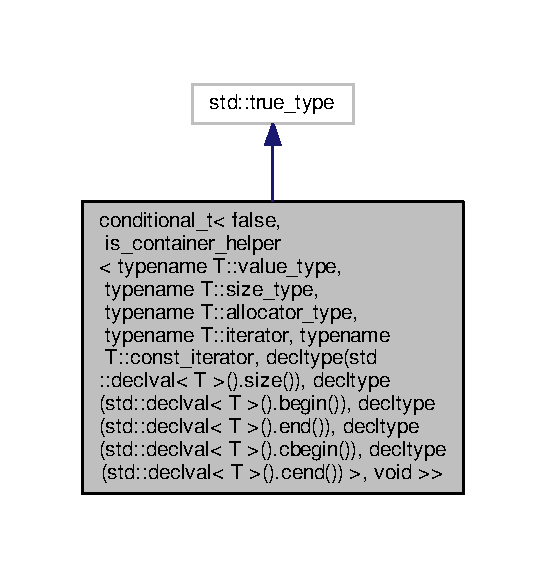
\includegraphics[width=262pt]{structis__container_3_01_t_00_01std_1_1conditional__t_3_01false_00_01is__container__helper_3_01t68dd0d5b6c9daa5bcca843ba638d58fd}
\end{center}
\end{figure}


Collaboration diagram for conditional\-\_\-t$<$ false, is\-\_\-container\-\_\-helper$<$ typename T\-:\-:value\-\_\-type, typename T\-:\-:size\-\_\-type, typename T\-:\-:allocator\-\_\-type, typename T\-:\-:iterator, typename T\-:\-:const\-\_\-iterator, decltype(std\-:\-:declval$<$ T $>$().size()), decltype(std\-:\-:declval$<$ T $>$().begin()), decltype(std\-:\-:declval$<$ T $>$().end()), decltype(std\-:\-:declval$<$ T $>$().cbegin()), decltype(std\-:\-:declval$<$ T $>$().cend()) $>$, void $>$$>$\-:
\nopagebreak
\begin{figure}[H]
\begin{center}
\leavevmode
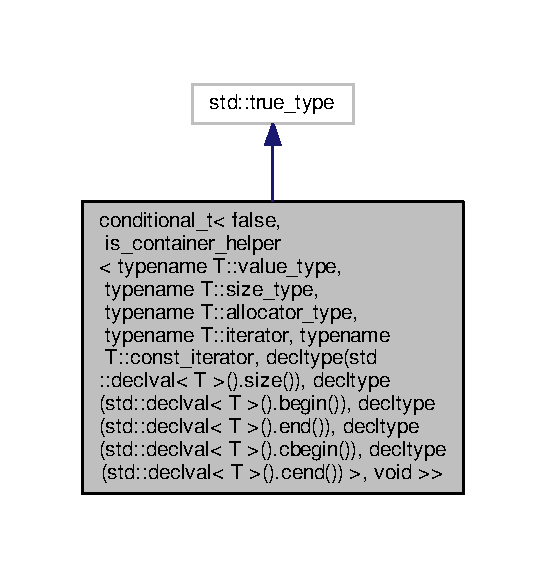
\includegraphics[width=262pt]{structis__container_3_01_t_00_01std_1_1conditional__t_3_01false_00_01is__container__helper_3_01t6d3f177557a3c17216cc20edaf3f7e80}
\end{center}
\end{figure}


The documentation for this struct was generated from the following file\-:\begin{DoxyCompactItemize}
\item 
include/\hyperlink{traits_8h}{traits.\-h}\end{DoxyCompactItemize}

\hypertarget{structis__container}{\section{is\-\_\-container$<$ T, \-\_\- $>$ Struct Template Reference}
\label{structis__container}\index{is\-\_\-container$<$ T, \-\_\- $>$@{is\-\_\-container$<$ T, \-\_\- $>$}}
}


{\ttfamily \#include $<$traits.\-h$>$}



Inheritance diagram for is\-\_\-container$<$ T, \-\_\- $>$\-:
\nopagebreak
\begin{figure}[H]
\begin{center}
\leavevmode
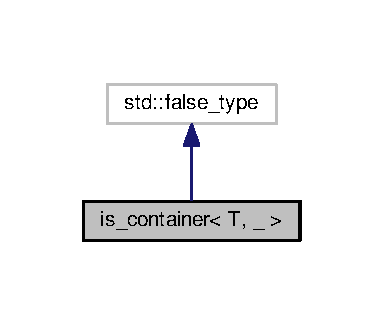
\includegraphics[width=184pt]{structis__container__inherit__graph}
\end{center}
\end{figure}


Collaboration diagram for is\-\_\-container$<$ T, \-\_\- $>$\-:
\nopagebreak
\begin{figure}[H]
\begin{center}
\leavevmode
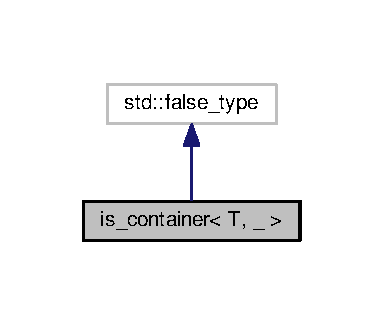
\includegraphics[width=184pt]{structis__container__coll__graph}
\end{center}
\end{figure}


The documentation for this struct was generated from the following file\-:\begin{DoxyCompactItemize}
\item 
include/\hyperlink{traits_8h}{traits.\-h}\end{DoxyCompactItemize}

\hypertarget{structis__container__helper}{\section{is\-\_\-container\-\_\-helper$<$ Ts $>$ Struct Template Reference}
\label{structis__container__helper}\index{is\-\_\-container\-\_\-helper$<$ Ts $>$@{is\-\_\-container\-\_\-helper$<$ Ts $>$}}
}


{\ttfamily \#include $<$traits.\-h$>$}



The documentation for this struct was generated from the following file\-:\begin{DoxyCompactItemize}
\item 
include/\hyperlink{traits_8h}{traits.\-h}\end{DoxyCompactItemize}

\chapter{File Documentation}
\hypertarget{_c_make_c_compiler_id_8c}{\section{C\-Make\-Files/3.9.2/\-Compiler\-Id\-C/\-C\-Make\-C\-Compiler\-Id.c File Reference}
\label{_c_make_c_compiler_id_8c}\index{C\-Make\-Files/3.\-9.\-2/\-Compiler\-Id\-C/\-C\-Make\-C\-Compiler\-Id.\-c@{C\-Make\-Files/3.\-9.\-2/\-Compiler\-Id\-C/\-C\-Make\-C\-Compiler\-Id.\-c}}
}
\subsection*{Macros}
\begin{DoxyCompactItemize}
\item 
\#define \hyperlink{_c_make_c_compiler_id_8c_a81dee0709ded976b2e0319239f72d174}{C\-O\-M\-P\-I\-L\-E\-R\-\_\-\-I\-D}~\char`\"{}\char`\"{}
\item 
\#define \hyperlink{_c_make_c_compiler_id_8c_a2ae9b72bb13abaabfcf2ee0ba7d3fa1d}{S\-T\-R\-I\-N\-G\-I\-F\-Y\-\_\-\-H\-E\-L\-P\-E\-R}(X)~\#X
\item 
\#define \hyperlink{_c_make_c_compiler_id_8c_a43e1cad902b6477bec893cb6430bd6c8}{S\-T\-R\-I\-N\-G\-I\-F\-Y}(X)~\hyperlink{_c_make_c_x_x_compiler_id_8cpp_a2ae9b72bb13abaabfcf2ee0ba7d3fa1d}{S\-T\-R\-I\-N\-G\-I\-F\-Y\-\_\-\-H\-E\-L\-P\-E\-R}(X)
\item 
\#define \hyperlink{_c_make_c_compiler_id_8c_adbc5372f40838899018fadbc89bd588b}{P\-L\-A\-T\-F\-O\-R\-M\-\_\-\-I\-D}
\item 
\#define \hyperlink{_c_make_c_compiler_id_8c_aba35d0d200deaeb06aee95ca297acb28}{A\-R\-C\-H\-I\-T\-E\-C\-T\-U\-R\-E\-\_\-\-I\-D}
\item 
\#define \hyperlink{_c_make_c_compiler_id_8c_ad1280362da42492bbc11aa78cbf776ad}{D\-E\-C}(n)
\item 
\#define \hyperlink{_c_make_c_compiler_id_8c_a46d5d95daa1bef867bd0179594310ed5}{H\-E\-X}(n)
\item 
\#define \hyperlink{_c_make_c_compiler_id_8c_a07f8e5783674099cd7f5110e22a78cdb}{C\-\_\-\-D\-I\-A\-L\-E\-C\-T}
\end{DoxyCompactItemize}
\subsection*{Functions}
\begin{DoxyCompactItemize}
\item 
int \hyperlink{_c_make_c_compiler_id_8c_a0ddf1224851353fc92bfbff6f499fa97}{main} (int argc, char $\ast$argv\mbox{[}$\,$\mbox{]})
\end{DoxyCompactItemize}
\subsection*{Variables}
\begin{DoxyCompactItemize}
\item 
char const $\ast$ \hyperlink{_c_make_c_compiler_id_8c_a4b0efeb7a5d59313986b3a0390f050f6}{info\-\_\-compiler} = \char`\"{}I\-N\-F\-O\char`\"{} \char`\"{}\-:\char`\"{} \char`\"{}compiler\mbox{[}\char`\"{} C\-O\-M\-P\-I\-L\-E\-R\-\_\-\-I\-D \char`\"{}\mbox{]}\char`\"{}
\item 
char const $\ast$ \hyperlink{_c_make_c_compiler_id_8c_a2321403dee54ee23f0c2fa849c60f7d4}{info\-\_\-platform} = \char`\"{}I\-N\-F\-O\char`\"{} \char`\"{}\-:\char`\"{} \char`\"{}platform\mbox{[}\char`\"{} P\-L\-A\-T\-F\-O\-R\-M\-\_\-\-I\-D \char`\"{}\mbox{]}\char`\"{}
\item 
char const $\ast$ \hyperlink{_c_make_c_compiler_id_8c_a59647e99d304ed33b15cb284c27ed391}{info\-\_\-arch} = \char`\"{}I\-N\-F\-O\char`\"{} \char`\"{}\-:\char`\"{} \char`\"{}arch\mbox{[}\char`\"{} A\-R\-C\-H\-I\-T\-E\-C\-T\-U\-R\-E\-\_\-\-I\-D \char`\"{}\mbox{]}\char`\"{}
\item 
const char $\ast$ \hyperlink{_c_make_c_compiler_id_8c_a1ce162bad2fe6966ac8b33cc19e120b8}{info\-\_\-language\-\_\-dialect\-\_\-default}
\end{DoxyCompactItemize}


\subsection{Macro Definition Documentation}
\hypertarget{_c_make_c_compiler_id_8c_aba35d0d200deaeb06aee95ca297acb28}{\index{C\-Make\-C\-Compiler\-Id.\-c@{C\-Make\-C\-Compiler\-Id.\-c}!A\-R\-C\-H\-I\-T\-E\-C\-T\-U\-R\-E\-\_\-\-I\-D@{A\-R\-C\-H\-I\-T\-E\-C\-T\-U\-R\-E\-\_\-\-I\-D}}
\index{A\-R\-C\-H\-I\-T\-E\-C\-T\-U\-R\-E\-\_\-\-I\-D@{A\-R\-C\-H\-I\-T\-E\-C\-T\-U\-R\-E\-\_\-\-I\-D}!CMakeCCompilerId.c@{C\-Make\-C\-Compiler\-Id.\-c}}
\subsubsection[{A\-R\-C\-H\-I\-T\-E\-C\-T\-U\-R\-E\-\_\-\-I\-D}]{\setlength{\rightskip}{0pt plus 5cm}\#define A\-R\-C\-H\-I\-T\-E\-C\-T\-U\-R\-E\-\_\-\-I\-D}}\label{_c_make_c_compiler_id_8c_aba35d0d200deaeb06aee95ca297acb28}
\hypertarget{_c_make_c_compiler_id_8c_a07f8e5783674099cd7f5110e22a78cdb}{\index{C\-Make\-C\-Compiler\-Id.\-c@{C\-Make\-C\-Compiler\-Id.\-c}!C\-\_\-\-D\-I\-A\-L\-E\-C\-T@{C\-\_\-\-D\-I\-A\-L\-E\-C\-T}}
\index{C\-\_\-\-D\-I\-A\-L\-E\-C\-T@{C\-\_\-\-D\-I\-A\-L\-E\-C\-T}!CMakeCCompilerId.c@{C\-Make\-C\-Compiler\-Id.\-c}}
\subsubsection[{C\-\_\-\-D\-I\-A\-L\-E\-C\-T}]{\setlength{\rightskip}{0pt plus 5cm}\#define C\-\_\-\-D\-I\-A\-L\-E\-C\-T}}\label{_c_make_c_compiler_id_8c_a07f8e5783674099cd7f5110e22a78cdb}
\hypertarget{_c_make_c_compiler_id_8c_a81dee0709ded976b2e0319239f72d174}{\index{C\-Make\-C\-Compiler\-Id.\-c@{C\-Make\-C\-Compiler\-Id.\-c}!C\-O\-M\-P\-I\-L\-E\-R\-\_\-\-I\-D@{C\-O\-M\-P\-I\-L\-E\-R\-\_\-\-I\-D}}
\index{C\-O\-M\-P\-I\-L\-E\-R\-\_\-\-I\-D@{C\-O\-M\-P\-I\-L\-E\-R\-\_\-\-I\-D}!CMakeCCompilerId.c@{C\-Make\-C\-Compiler\-Id.\-c}}
\subsubsection[{C\-O\-M\-P\-I\-L\-E\-R\-\_\-\-I\-D}]{\setlength{\rightskip}{0pt plus 5cm}\#define C\-O\-M\-P\-I\-L\-E\-R\-\_\-\-I\-D~\char`\"{}\char`\"{}}}\label{_c_make_c_compiler_id_8c_a81dee0709ded976b2e0319239f72d174}
\hypertarget{_c_make_c_compiler_id_8c_ad1280362da42492bbc11aa78cbf776ad}{\index{C\-Make\-C\-Compiler\-Id.\-c@{C\-Make\-C\-Compiler\-Id.\-c}!D\-E\-C@{D\-E\-C}}
\index{D\-E\-C@{D\-E\-C}!CMakeCCompilerId.c@{C\-Make\-C\-Compiler\-Id.\-c}}
\subsubsection[{D\-E\-C}]{\setlength{\rightskip}{0pt plus 5cm}\#define D\-E\-C(
\begin{DoxyParamCaption}
\item[{}]{n}
\end{DoxyParamCaption}
)}}\label{_c_make_c_compiler_id_8c_ad1280362da42492bbc11aa78cbf776ad}
{\bfseries Value\-:}
\begin{DoxyCode}
(\textcolor{charliteral}{'0'} + (((n) / 10000000)%10)), \(\backslash\)
  (\textcolor{charliteral}{'0'} + (((n) / 1000000)%10)),  \(\backslash\)
  (\textcolor{charliteral}{'0'} + (((n) / 100000)%10)),   \(\backslash\)
  (\textcolor{charliteral}{'0'} + (((n) / 10000)%10)),    \(\backslash\)
  (\textcolor{charliteral}{'0'} + (((n) / 1000)%10)),     \(\backslash\)
  (\textcolor{charliteral}{'0'} + (((n) / 100)%10)),      \(\backslash\)
  (\textcolor{charliteral}{'0'} + (((n) / 10)%10)),       \(\backslash\)
  (\textcolor{charliteral}{'0'} +  ((n) % 10))
\end{DoxyCode}
\hypertarget{_c_make_c_compiler_id_8c_a46d5d95daa1bef867bd0179594310ed5}{\index{C\-Make\-C\-Compiler\-Id.\-c@{C\-Make\-C\-Compiler\-Id.\-c}!H\-E\-X@{H\-E\-X}}
\index{H\-E\-X@{H\-E\-X}!CMakeCCompilerId.c@{C\-Make\-C\-Compiler\-Id.\-c}}
\subsubsection[{H\-E\-X}]{\setlength{\rightskip}{0pt plus 5cm}\#define H\-E\-X(
\begin{DoxyParamCaption}
\item[{}]{n}
\end{DoxyParamCaption}
)}}\label{_c_make_c_compiler_id_8c_a46d5d95daa1bef867bd0179594310ed5}
{\bfseries Value\-:}
\begin{DoxyCode}
(\textcolor{charliteral}{'0'} + ((n)>>28 & 0xF)), \(\backslash\)
  (\textcolor{charliteral}{'0'} + ((n)>>24 & 0xF)), \(\backslash\)
  (\textcolor{charliteral}{'0'} + ((n)>>20 & 0xF)), \(\backslash\)
  (\textcolor{charliteral}{'0'} + ((n)>>16 & 0xF)), \(\backslash\)
  (\textcolor{charliteral}{'0'} + ((n)>>12 & 0xF)), \(\backslash\)
  (\textcolor{charliteral}{'0'} + ((n)>>8  & 0xF)), \(\backslash\)
  (\textcolor{charliteral}{'0'} + ((n)>>4  & 0xF)), \(\backslash\)
  (\textcolor{charliteral}{'0'} + ((n)     & 0xF))
\end{DoxyCode}
\hypertarget{_c_make_c_compiler_id_8c_adbc5372f40838899018fadbc89bd588b}{\index{C\-Make\-C\-Compiler\-Id.\-c@{C\-Make\-C\-Compiler\-Id.\-c}!P\-L\-A\-T\-F\-O\-R\-M\-\_\-\-I\-D@{P\-L\-A\-T\-F\-O\-R\-M\-\_\-\-I\-D}}
\index{P\-L\-A\-T\-F\-O\-R\-M\-\_\-\-I\-D@{P\-L\-A\-T\-F\-O\-R\-M\-\_\-\-I\-D}!CMakeCCompilerId.c@{C\-Make\-C\-Compiler\-Id.\-c}}
\subsubsection[{P\-L\-A\-T\-F\-O\-R\-M\-\_\-\-I\-D}]{\setlength{\rightskip}{0pt plus 5cm}\#define P\-L\-A\-T\-F\-O\-R\-M\-\_\-\-I\-D}}\label{_c_make_c_compiler_id_8c_adbc5372f40838899018fadbc89bd588b}
\hypertarget{_c_make_c_compiler_id_8c_a43e1cad902b6477bec893cb6430bd6c8}{\index{C\-Make\-C\-Compiler\-Id.\-c@{C\-Make\-C\-Compiler\-Id.\-c}!S\-T\-R\-I\-N\-G\-I\-F\-Y@{S\-T\-R\-I\-N\-G\-I\-F\-Y}}
\index{S\-T\-R\-I\-N\-G\-I\-F\-Y@{S\-T\-R\-I\-N\-G\-I\-F\-Y}!CMakeCCompilerId.c@{C\-Make\-C\-Compiler\-Id.\-c}}
\subsubsection[{S\-T\-R\-I\-N\-G\-I\-F\-Y}]{\setlength{\rightskip}{0pt plus 5cm}\#define S\-T\-R\-I\-N\-G\-I\-F\-Y(
\begin{DoxyParamCaption}
\item[{}]{X}
\end{DoxyParamCaption}
)~{\bf S\-T\-R\-I\-N\-G\-I\-F\-Y\-\_\-\-H\-E\-L\-P\-E\-R}(X)}}\label{_c_make_c_compiler_id_8c_a43e1cad902b6477bec893cb6430bd6c8}
\hypertarget{_c_make_c_compiler_id_8c_a2ae9b72bb13abaabfcf2ee0ba7d3fa1d}{\index{C\-Make\-C\-Compiler\-Id.\-c@{C\-Make\-C\-Compiler\-Id.\-c}!S\-T\-R\-I\-N\-G\-I\-F\-Y\-\_\-\-H\-E\-L\-P\-E\-R@{S\-T\-R\-I\-N\-G\-I\-F\-Y\-\_\-\-H\-E\-L\-P\-E\-R}}
\index{S\-T\-R\-I\-N\-G\-I\-F\-Y\-\_\-\-H\-E\-L\-P\-E\-R@{S\-T\-R\-I\-N\-G\-I\-F\-Y\-\_\-\-H\-E\-L\-P\-E\-R}!CMakeCCompilerId.c@{C\-Make\-C\-Compiler\-Id.\-c}}
\subsubsection[{S\-T\-R\-I\-N\-G\-I\-F\-Y\-\_\-\-H\-E\-L\-P\-E\-R}]{\setlength{\rightskip}{0pt plus 5cm}\#define S\-T\-R\-I\-N\-G\-I\-F\-Y\-\_\-\-H\-E\-L\-P\-E\-R(
\begin{DoxyParamCaption}
\item[{}]{X}
\end{DoxyParamCaption}
)~\#X}}\label{_c_make_c_compiler_id_8c_a2ae9b72bb13abaabfcf2ee0ba7d3fa1d}


\subsection{Function Documentation}
\hypertarget{_c_make_c_compiler_id_8c_a0ddf1224851353fc92bfbff6f499fa97}{\index{C\-Make\-C\-Compiler\-Id.\-c@{C\-Make\-C\-Compiler\-Id.\-c}!main@{main}}
\index{main@{main}!CMakeCCompilerId.c@{C\-Make\-C\-Compiler\-Id.\-c}}
\subsubsection[{main}]{\setlength{\rightskip}{0pt plus 5cm}int main (
\begin{DoxyParamCaption}
\item[{int}]{argc, }
\item[{char $\ast$}]{argv\mbox{[}$\,$\mbox{]}}
\end{DoxyParamCaption}
)}}\label{_c_make_c_compiler_id_8c_a0ddf1224851353fc92bfbff6f499fa97}


\subsection{Variable Documentation}
\hypertarget{_c_make_c_compiler_id_8c_a59647e99d304ed33b15cb284c27ed391}{\index{C\-Make\-C\-Compiler\-Id.\-c@{C\-Make\-C\-Compiler\-Id.\-c}!info\-\_\-arch@{info\-\_\-arch}}
\index{info\-\_\-arch@{info\-\_\-arch}!CMakeCCompilerId.c@{C\-Make\-C\-Compiler\-Id.\-c}}
\subsubsection[{info\-\_\-arch}]{\setlength{\rightskip}{0pt plus 5cm}char const$\ast$ info\-\_\-arch = \char`\"{}I\-N\-F\-O\char`\"{} \char`\"{}\-:\char`\"{} \char`\"{}arch\mbox{[}\char`\"{} A\-R\-C\-H\-I\-T\-E\-C\-T\-U\-R\-E\-\_\-\-I\-D \char`\"{}\mbox{]}\char`\"{}}}\label{_c_make_c_compiler_id_8c_a59647e99d304ed33b15cb284c27ed391}
\hypertarget{_c_make_c_compiler_id_8c_a4b0efeb7a5d59313986b3a0390f050f6}{\index{C\-Make\-C\-Compiler\-Id.\-c@{C\-Make\-C\-Compiler\-Id.\-c}!info\-\_\-compiler@{info\-\_\-compiler}}
\index{info\-\_\-compiler@{info\-\_\-compiler}!CMakeCCompilerId.c@{C\-Make\-C\-Compiler\-Id.\-c}}
\subsubsection[{info\-\_\-compiler}]{\setlength{\rightskip}{0pt plus 5cm}char const$\ast$ info\-\_\-compiler = \char`\"{}I\-N\-F\-O\char`\"{} \char`\"{}\-:\char`\"{} \char`\"{}compiler\mbox{[}\char`\"{} C\-O\-M\-P\-I\-L\-E\-R\-\_\-\-I\-D \char`\"{}\mbox{]}\char`\"{}}}\label{_c_make_c_compiler_id_8c_a4b0efeb7a5d59313986b3a0390f050f6}
\hypertarget{_c_make_c_compiler_id_8c_a1ce162bad2fe6966ac8b33cc19e120b8}{\index{C\-Make\-C\-Compiler\-Id.\-c@{C\-Make\-C\-Compiler\-Id.\-c}!info\-\_\-language\-\_\-dialect\-\_\-default@{info\-\_\-language\-\_\-dialect\-\_\-default}}
\index{info\-\_\-language\-\_\-dialect\-\_\-default@{info\-\_\-language\-\_\-dialect\-\_\-default}!CMakeCCompilerId.c@{C\-Make\-C\-Compiler\-Id.\-c}}
\subsubsection[{info\-\_\-language\-\_\-dialect\-\_\-default}]{\setlength{\rightskip}{0pt plus 5cm}const char$\ast$ info\-\_\-language\-\_\-dialect\-\_\-default}}\label{_c_make_c_compiler_id_8c_a1ce162bad2fe6966ac8b33cc19e120b8}
{\bfseries Initial value\-:}
\begin{DoxyCode}
=
  \textcolor{stringliteral}{"INFO"} \textcolor{stringliteral}{":"} \textcolor{stringliteral}{"dialect\_default["} \hyperlink{_c_make_c_compiler_id_8c_a07f8e5783674099cd7f5110e22a78cdb}{C\_DIALECT} \textcolor{stringliteral}{"]"}
\end{DoxyCode}
\hypertarget{_c_make_c_compiler_id_8c_a2321403dee54ee23f0c2fa849c60f7d4}{\index{C\-Make\-C\-Compiler\-Id.\-c@{C\-Make\-C\-Compiler\-Id.\-c}!info\-\_\-platform@{info\-\_\-platform}}
\index{info\-\_\-platform@{info\-\_\-platform}!CMakeCCompilerId.c@{C\-Make\-C\-Compiler\-Id.\-c}}
\subsubsection[{info\-\_\-platform}]{\setlength{\rightskip}{0pt plus 5cm}char const$\ast$ info\-\_\-platform = \char`\"{}I\-N\-F\-O\char`\"{} \char`\"{}\-:\char`\"{} \char`\"{}platform\mbox{[}\char`\"{} P\-L\-A\-T\-F\-O\-R\-M\-\_\-\-I\-D \char`\"{}\mbox{]}\char`\"{}}}\label{_c_make_c_compiler_id_8c_a2321403dee54ee23f0c2fa849c60f7d4}

\hypertarget{_c_make_c_x_x_compiler_id_8cpp}{\section{C\-Make\-Files/3.9.2/\-Compiler\-Id\-C\-X\-X/\-C\-Make\-C\-X\-X\-Compiler\-Id.cpp File Reference}
\label{_c_make_c_x_x_compiler_id_8cpp}\index{C\-Make\-Files/3.\-9.\-2/\-Compiler\-Id\-C\-X\-X/\-C\-Make\-C\-X\-X\-Compiler\-Id.\-cpp@{C\-Make\-Files/3.\-9.\-2/\-Compiler\-Id\-C\-X\-X/\-C\-Make\-C\-X\-X\-Compiler\-Id.\-cpp}}
}
\subsection*{Macros}
\begin{DoxyCompactItemize}
\item 
\#define \hyperlink{_c_make_c_x_x_compiler_id_8cpp_a81dee0709ded976b2e0319239f72d174}{C\-O\-M\-P\-I\-L\-E\-R\-\_\-\-I\-D}~\char`\"{}\char`\"{}
\item 
\#define \hyperlink{_c_make_c_x_x_compiler_id_8cpp_a2ae9b72bb13abaabfcf2ee0ba7d3fa1d}{S\-T\-R\-I\-N\-G\-I\-F\-Y\-\_\-\-H\-E\-L\-P\-E\-R}(X)~\#X
\item 
\#define \hyperlink{_c_make_c_x_x_compiler_id_8cpp_a43e1cad902b6477bec893cb6430bd6c8}{S\-T\-R\-I\-N\-G\-I\-F\-Y}(X)~\hyperlink{_c_make_c_x_x_compiler_id_8cpp_a2ae9b72bb13abaabfcf2ee0ba7d3fa1d}{S\-T\-R\-I\-N\-G\-I\-F\-Y\-\_\-\-H\-E\-L\-P\-E\-R}(X)
\item 
\#define \hyperlink{_c_make_c_x_x_compiler_id_8cpp_adbc5372f40838899018fadbc89bd588b}{P\-L\-A\-T\-F\-O\-R\-M\-\_\-\-I\-D}
\item 
\#define \hyperlink{_c_make_c_x_x_compiler_id_8cpp_aba35d0d200deaeb06aee95ca297acb28}{A\-R\-C\-H\-I\-T\-E\-C\-T\-U\-R\-E\-\_\-\-I\-D}
\item 
\#define \hyperlink{_c_make_c_x_x_compiler_id_8cpp_ad1280362da42492bbc11aa78cbf776ad}{D\-E\-C}(n)
\item 
\#define \hyperlink{_c_make_c_x_x_compiler_id_8cpp_a46d5d95daa1bef867bd0179594310ed5}{H\-E\-X}(n)
\end{DoxyCompactItemize}
\subsection*{Functions}
\begin{DoxyCompactItemize}
\item 
int \hyperlink{_c_make_c_x_x_compiler_id_8cpp_a0ddf1224851353fc92bfbff6f499fa97}{main} (int argc, char $\ast$argv\mbox{[}$\,$\mbox{]})
\end{DoxyCompactItemize}
\subsection*{Variables}
\begin{DoxyCompactItemize}
\item 
char const $\ast$ \hyperlink{_c_make_c_x_x_compiler_id_8cpp_a4b0efeb7a5d59313986b3a0390f050f6}{info\-\_\-compiler} = \char`\"{}I\-N\-F\-O\char`\"{} \char`\"{}\-:\char`\"{} \char`\"{}compiler\mbox{[}\char`\"{} C\-O\-M\-P\-I\-L\-E\-R\-\_\-\-I\-D \char`\"{}\mbox{]}\char`\"{}
\item 
char const $\ast$ \hyperlink{_c_make_c_x_x_compiler_id_8cpp_a2321403dee54ee23f0c2fa849c60f7d4}{info\-\_\-platform} = \char`\"{}I\-N\-F\-O\char`\"{} \char`\"{}\-:\char`\"{} \char`\"{}platform\mbox{[}\char`\"{} P\-L\-A\-T\-F\-O\-R\-M\-\_\-\-I\-D \char`\"{}\mbox{]}\char`\"{}
\item 
char const $\ast$ \hyperlink{_c_make_c_x_x_compiler_id_8cpp_a59647e99d304ed33b15cb284c27ed391}{info\-\_\-arch} = \char`\"{}I\-N\-F\-O\char`\"{} \char`\"{}\-:\char`\"{} \char`\"{}arch\mbox{[}\char`\"{} A\-R\-C\-H\-I\-T\-E\-C\-T\-U\-R\-E\-\_\-\-I\-D \char`\"{}\mbox{]}\char`\"{}
\item 
const char $\ast$ \hyperlink{_c_make_c_x_x_compiler_id_8cpp_a1ce162bad2fe6966ac8b33cc19e120b8}{info\-\_\-language\-\_\-dialect\-\_\-default}
\end{DoxyCompactItemize}


\subsection{Macro Definition Documentation}
\hypertarget{_c_make_c_x_x_compiler_id_8cpp_aba35d0d200deaeb06aee95ca297acb28}{\index{C\-Make\-C\-X\-X\-Compiler\-Id.\-cpp@{C\-Make\-C\-X\-X\-Compiler\-Id.\-cpp}!A\-R\-C\-H\-I\-T\-E\-C\-T\-U\-R\-E\-\_\-\-I\-D@{A\-R\-C\-H\-I\-T\-E\-C\-T\-U\-R\-E\-\_\-\-I\-D}}
\index{A\-R\-C\-H\-I\-T\-E\-C\-T\-U\-R\-E\-\_\-\-I\-D@{A\-R\-C\-H\-I\-T\-E\-C\-T\-U\-R\-E\-\_\-\-I\-D}!CMakeCXXCompilerId.cpp@{C\-Make\-C\-X\-X\-Compiler\-Id.\-cpp}}
\subsubsection[{A\-R\-C\-H\-I\-T\-E\-C\-T\-U\-R\-E\-\_\-\-I\-D}]{\setlength{\rightskip}{0pt plus 5cm}\#define A\-R\-C\-H\-I\-T\-E\-C\-T\-U\-R\-E\-\_\-\-I\-D}}\label{_c_make_c_x_x_compiler_id_8cpp_aba35d0d200deaeb06aee95ca297acb28}
\hypertarget{_c_make_c_x_x_compiler_id_8cpp_a81dee0709ded976b2e0319239f72d174}{\index{C\-Make\-C\-X\-X\-Compiler\-Id.\-cpp@{C\-Make\-C\-X\-X\-Compiler\-Id.\-cpp}!C\-O\-M\-P\-I\-L\-E\-R\-\_\-\-I\-D@{C\-O\-M\-P\-I\-L\-E\-R\-\_\-\-I\-D}}
\index{C\-O\-M\-P\-I\-L\-E\-R\-\_\-\-I\-D@{C\-O\-M\-P\-I\-L\-E\-R\-\_\-\-I\-D}!CMakeCXXCompilerId.cpp@{C\-Make\-C\-X\-X\-Compiler\-Id.\-cpp}}
\subsubsection[{C\-O\-M\-P\-I\-L\-E\-R\-\_\-\-I\-D}]{\setlength{\rightskip}{0pt plus 5cm}\#define C\-O\-M\-P\-I\-L\-E\-R\-\_\-\-I\-D~\char`\"{}\char`\"{}}}\label{_c_make_c_x_x_compiler_id_8cpp_a81dee0709ded976b2e0319239f72d174}
\hypertarget{_c_make_c_x_x_compiler_id_8cpp_ad1280362da42492bbc11aa78cbf776ad}{\index{C\-Make\-C\-X\-X\-Compiler\-Id.\-cpp@{C\-Make\-C\-X\-X\-Compiler\-Id.\-cpp}!D\-E\-C@{D\-E\-C}}
\index{D\-E\-C@{D\-E\-C}!CMakeCXXCompilerId.cpp@{C\-Make\-C\-X\-X\-Compiler\-Id.\-cpp}}
\subsubsection[{D\-E\-C}]{\setlength{\rightskip}{0pt plus 5cm}\#define D\-E\-C(
\begin{DoxyParamCaption}
\item[{}]{n}
\end{DoxyParamCaption}
)}}\label{_c_make_c_x_x_compiler_id_8cpp_ad1280362da42492bbc11aa78cbf776ad}
{\bfseries Value\-:}
\begin{DoxyCode}
(\textcolor{charliteral}{'0'} + (((n) / 10000000)%10)), \(\backslash\)
  (\textcolor{charliteral}{'0'} + (((n) / 1000000)%10)),  \(\backslash\)
  (\textcolor{charliteral}{'0'} + (((n) / 100000)%10)),   \(\backslash\)
  (\textcolor{charliteral}{'0'} + (((n) / 10000)%10)),    \(\backslash\)
  (\textcolor{charliteral}{'0'} + (((n) / 1000)%10)),     \(\backslash\)
  (\textcolor{charliteral}{'0'} + (((n) / 100)%10)),      \(\backslash\)
  (\textcolor{charliteral}{'0'} + (((n) / 10)%10)),       \(\backslash\)
  (\textcolor{charliteral}{'0'} +  ((n) % 10))
\end{DoxyCode}
\hypertarget{_c_make_c_x_x_compiler_id_8cpp_a46d5d95daa1bef867bd0179594310ed5}{\index{C\-Make\-C\-X\-X\-Compiler\-Id.\-cpp@{C\-Make\-C\-X\-X\-Compiler\-Id.\-cpp}!H\-E\-X@{H\-E\-X}}
\index{H\-E\-X@{H\-E\-X}!CMakeCXXCompilerId.cpp@{C\-Make\-C\-X\-X\-Compiler\-Id.\-cpp}}
\subsubsection[{H\-E\-X}]{\setlength{\rightskip}{0pt plus 5cm}\#define H\-E\-X(
\begin{DoxyParamCaption}
\item[{}]{n}
\end{DoxyParamCaption}
)}}\label{_c_make_c_x_x_compiler_id_8cpp_a46d5d95daa1bef867bd0179594310ed5}
{\bfseries Value\-:}
\begin{DoxyCode}
(\textcolor{charliteral}{'0'} + ((n)>>28 & 0xF)), \(\backslash\)
  (\textcolor{charliteral}{'0'} + ((n)>>24 & 0xF)), \(\backslash\)
  (\textcolor{charliteral}{'0'} + ((n)>>20 & 0xF)), \(\backslash\)
  (\textcolor{charliteral}{'0'} + ((n)>>16 & 0xF)), \(\backslash\)
  (\textcolor{charliteral}{'0'} + ((n)>>12 & 0xF)), \(\backslash\)
  (\textcolor{charliteral}{'0'} + ((n)>>8  & 0xF)), \(\backslash\)
  (\textcolor{charliteral}{'0'} + ((n)>>4  & 0xF)), \(\backslash\)
  (\textcolor{charliteral}{'0'} + ((n)     & 0xF))
\end{DoxyCode}
\hypertarget{_c_make_c_x_x_compiler_id_8cpp_adbc5372f40838899018fadbc89bd588b}{\index{C\-Make\-C\-X\-X\-Compiler\-Id.\-cpp@{C\-Make\-C\-X\-X\-Compiler\-Id.\-cpp}!P\-L\-A\-T\-F\-O\-R\-M\-\_\-\-I\-D@{P\-L\-A\-T\-F\-O\-R\-M\-\_\-\-I\-D}}
\index{P\-L\-A\-T\-F\-O\-R\-M\-\_\-\-I\-D@{P\-L\-A\-T\-F\-O\-R\-M\-\_\-\-I\-D}!CMakeCXXCompilerId.cpp@{C\-Make\-C\-X\-X\-Compiler\-Id.\-cpp}}
\subsubsection[{P\-L\-A\-T\-F\-O\-R\-M\-\_\-\-I\-D}]{\setlength{\rightskip}{0pt plus 5cm}\#define P\-L\-A\-T\-F\-O\-R\-M\-\_\-\-I\-D}}\label{_c_make_c_x_x_compiler_id_8cpp_adbc5372f40838899018fadbc89bd588b}
\hypertarget{_c_make_c_x_x_compiler_id_8cpp_a43e1cad902b6477bec893cb6430bd6c8}{\index{C\-Make\-C\-X\-X\-Compiler\-Id.\-cpp@{C\-Make\-C\-X\-X\-Compiler\-Id.\-cpp}!S\-T\-R\-I\-N\-G\-I\-F\-Y@{S\-T\-R\-I\-N\-G\-I\-F\-Y}}
\index{S\-T\-R\-I\-N\-G\-I\-F\-Y@{S\-T\-R\-I\-N\-G\-I\-F\-Y}!CMakeCXXCompilerId.cpp@{C\-Make\-C\-X\-X\-Compiler\-Id.\-cpp}}
\subsubsection[{S\-T\-R\-I\-N\-G\-I\-F\-Y}]{\setlength{\rightskip}{0pt plus 5cm}\#define S\-T\-R\-I\-N\-G\-I\-F\-Y(
\begin{DoxyParamCaption}
\item[{}]{X}
\end{DoxyParamCaption}
)~{\bf S\-T\-R\-I\-N\-G\-I\-F\-Y\-\_\-\-H\-E\-L\-P\-E\-R}(X)}}\label{_c_make_c_x_x_compiler_id_8cpp_a43e1cad902b6477bec893cb6430bd6c8}
\hypertarget{_c_make_c_x_x_compiler_id_8cpp_a2ae9b72bb13abaabfcf2ee0ba7d3fa1d}{\index{C\-Make\-C\-X\-X\-Compiler\-Id.\-cpp@{C\-Make\-C\-X\-X\-Compiler\-Id.\-cpp}!S\-T\-R\-I\-N\-G\-I\-F\-Y\-\_\-\-H\-E\-L\-P\-E\-R@{S\-T\-R\-I\-N\-G\-I\-F\-Y\-\_\-\-H\-E\-L\-P\-E\-R}}
\index{S\-T\-R\-I\-N\-G\-I\-F\-Y\-\_\-\-H\-E\-L\-P\-E\-R@{S\-T\-R\-I\-N\-G\-I\-F\-Y\-\_\-\-H\-E\-L\-P\-E\-R}!CMakeCXXCompilerId.cpp@{C\-Make\-C\-X\-X\-Compiler\-Id.\-cpp}}
\subsubsection[{S\-T\-R\-I\-N\-G\-I\-F\-Y\-\_\-\-H\-E\-L\-P\-E\-R}]{\setlength{\rightskip}{0pt plus 5cm}\#define S\-T\-R\-I\-N\-G\-I\-F\-Y\-\_\-\-H\-E\-L\-P\-E\-R(
\begin{DoxyParamCaption}
\item[{}]{X}
\end{DoxyParamCaption}
)~\#X}}\label{_c_make_c_x_x_compiler_id_8cpp_a2ae9b72bb13abaabfcf2ee0ba7d3fa1d}


\subsection{Function Documentation}
\hypertarget{_c_make_c_x_x_compiler_id_8cpp_a0ddf1224851353fc92bfbff6f499fa97}{\index{C\-Make\-C\-X\-X\-Compiler\-Id.\-cpp@{C\-Make\-C\-X\-X\-Compiler\-Id.\-cpp}!main@{main}}
\index{main@{main}!CMakeCXXCompilerId.cpp@{C\-Make\-C\-X\-X\-Compiler\-Id.\-cpp}}
\subsubsection[{main}]{\setlength{\rightskip}{0pt plus 5cm}int main (
\begin{DoxyParamCaption}
\item[{int}]{argc, }
\item[{char $\ast$}]{argv\mbox{[}$\,$\mbox{]}}
\end{DoxyParamCaption}
)}}\label{_c_make_c_x_x_compiler_id_8cpp_a0ddf1224851353fc92bfbff6f499fa97}


\subsection{Variable Documentation}
\hypertarget{_c_make_c_x_x_compiler_id_8cpp_a59647e99d304ed33b15cb284c27ed391}{\index{C\-Make\-C\-X\-X\-Compiler\-Id.\-cpp@{C\-Make\-C\-X\-X\-Compiler\-Id.\-cpp}!info\-\_\-arch@{info\-\_\-arch}}
\index{info\-\_\-arch@{info\-\_\-arch}!CMakeCXXCompilerId.cpp@{C\-Make\-C\-X\-X\-Compiler\-Id.\-cpp}}
\subsubsection[{info\-\_\-arch}]{\setlength{\rightskip}{0pt plus 5cm}char const$\ast$ info\-\_\-arch = \char`\"{}I\-N\-F\-O\char`\"{} \char`\"{}\-:\char`\"{} \char`\"{}arch\mbox{[}\char`\"{} A\-R\-C\-H\-I\-T\-E\-C\-T\-U\-R\-E\-\_\-\-I\-D \char`\"{}\mbox{]}\char`\"{}}}\label{_c_make_c_x_x_compiler_id_8cpp_a59647e99d304ed33b15cb284c27ed391}
\hypertarget{_c_make_c_x_x_compiler_id_8cpp_a4b0efeb7a5d59313986b3a0390f050f6}{\index{C\-Make\-C\-X\-X\-Compiler\-Id.\-cpp@{C\-Make\-C\-X\-X\-Compiler\-Id.\-cpp}!info\-\_\-compiler@{info\-\_\-compiler}}
\index{info\-\_\-compiler@{info\-\_\-compiler}!CMakeCXXCompilerId.cpp@{C\-Make\-C\-X\-X\-Compiler\-Id.\-cpp}}
\subsubsection[{info\-\_\-compiler}]{\setlength{\rightskip}{0pt plus 5cm}char const$\ast$ info\-\_\-compiler = \char`\"{}I\-N\-F\-O\char`\"{} \char`\"{}\-:\char`\"{} \char`\"{}compiler\mbox{[}\char`\"{} C\-O\-M\-P\-I\-L\-E\-R\-\_\-\-I\-D \char`\"{}\mbox{]}\char`\"{}}}\label{_c_make_c_x_x_compiler_id_8cpp_a4b0efeb7a5d59313986b3a0390f050f6}
\hypertarget{_c_make_c_x_x_compiler_id_8cpp_a1ce162bad2fe6966ac8b33cc19e120b8}{\index{C\-Make\-C\-X\-X\-Compiler\-Id.\-cpp@{C\-Make\-C\-X\-X\-Compiler\-Id.\-cpp}!info\-\_\-language\-\_\-dialect\-\_\-default@{info\-\_\-language\-\_\-dialect\-\_\-default}}
\index{info\-\_\-language\-\_\-dialect\-\_\-default@{info\-\_\-language\-\_\-dialect\-\_\-default}!CMakeCXXCompilerId.cpp@{C\-Make\-C\-X\-X\-Compiler\-Id.\-cpp}}
\subsubsection[{info\-\_\-language\-\_\-dialect\-\_\-default}]{\setlength{\rightskip}{0pt plus 5cm}const char$\ast$ info\-\_\-language\-\_\-dialect\-\_\-default}}\label{_c_make_c_x_x_compiler_id_8cpp_a1ce162bad2fe6966ac8b33cc19e120b8}
{\bfseries Initial value\-:}
\begin{DoxyCode}
= \textcolor{stringliteral}{"INFO"} \textcolor{stringliteral}{":"} \textcolor{stringliteral}{"dialect\_default["}







  \textcolor{stringliteral}{"98"}

\textcolor{stringliteral}{"]"}
\end{DoxyCode}
\hypertarget{_c_make_c_x_x_compiler_id_8cpp_a2321403dee54ee23f0c2fa849c60f7d4}{\index{C\-Make\-C\-X\-X\-Compiler\-Id.\-cpp@{C\-Make\-C\-X\-X\-Compiler\-Id.\-cpp}!info\-\_\-platform@{info\-\_\-platform}}
\index{info\-\_\-platform@{info\-\_\-platform}!CMakeCXXCompilerId.cpp@{C\-Make\-C\-X\-X\-Compiler\-Id.\-cpp}}
\subsubsection[{info\-\_\-platform}]{\setlength{\rightskip}{0pt plus 5cm}char const$\ast$ info\-\_\-platform = \char`\"{}I\-N\-F\-O\char`\"{} \char`\"{}\-:\char`\"{} \char`\"{}platform\mbox{[}\char`\"{} P\-L\-A\-T\-F\-O\-R\-M\-\_\-\-I\-D \char`\"{}\mbox{]}\char`\"{}}}\label{_c_make_c_x_x_compiler_id_8cpp_a2321403dee54ee23f0c2fa849c60f7d4}

\hypertarget{feature__tests_8c}{\section{C\-Make\-Files/feature\-\_\-tests.c File Reference}
\label{feature__tests_8c}\index{C\-Make\-Files/feature\-\_\-tests.\-c@{C\-Make\-Files/feature\-\_\-tests.\-c}}
}
\subsection*{Functions}
\begin{DoxyCompactItemize}
\item 
int \hyperlink{feature__tests_8c_a3c04138a5bfe5d72780bb7e82a18e627}{main} (int argc, char $\ast$$\ast$argv)
\end{DoxyCompactItemize}
\subsection*{Variables}
\begin{DoxyCompactItemize}
\item 
const char \hyperlink{feature__tests_8c_a1582568e32f689337602a16bf8a5bff0}{features} \mbox{[}$\,$\mbox{]}
\end{DoxyCompactItemize}


\subsection{Function Documentation}
\hypertarget{feature__tests_8c_a3c04138a5bfe5d72780bb7e82a18e627}{\index{feature\-\_\-tests.\-c@{feature\-\_\-tests.\-c}!main@{main}}
\index{main@{main}!feature_tests.c@{feature\-\_\-tests.\-c}}
\subsubsection[{main}]{\setlength{\rightskip}{0pt plus 5cm}int main (
\begin{DoxyParamCaption}
\item[{int}]{argc, }
\item[{char $\ast$$\ast$}]{argv}
\end{DoxyParamCaption}
)}}\label{feature__tests_8c_a3c04138a5bfe5d72780bb7e82a18e627}


\subsection{Variable Documentation}
\hypertarget{feature__tests_8c_a1582568e32f689337602a16bf8a5bff0}{\index{feature\-\_\-tests.\-c@{feature\-\_\-tests.\-c}!features@{features}}
\index{features@{features}!feature_tests.c@{feature\-\_\-tests.\-c}}
\subsubsection[{features}]{\setlength{\rightskip}{0pt plus 5cm}const char features\mbox{[}$\,$\mbox{]}}}\label{feature__tests_8c_a1582568e32f689337602a16bf8a5bff0}

\hypertarget{feature__tests_8cxx}{\section{C\-Make\-Files/feature\-\_\-tests.cxx File Reference}
\label{feature__tests_8cxx}\index{C\-Make\-Files/feature\-\_\-tests.\-cxx@{C\-Make\-Files/feature\-\_\-tests.\-cxx}}
}
\subsection*{Functions}
\begin{DoxyCompactItemize}
\item 
int \hyperlink{feature__tests_8cxx_a3c04138a5bfe5d72780bb7e82a18e627}{main} (int argc, char $\ast$$\ast$argv)
\end{DoxyCompactItemize}
\subsection*{Variables}
\begin{DoxyCompactItemize}
\item 
const char \hyperlink{feature__tests_8cxx_a1582568e32f689337602a16bf8a5bff0}{features} \mbox{[}$\,$\mbox{]}
\end{DoxyCompactItemize}


\subsection{Function Documentation}
\hypertarget{feature__tests_8cxx_a3c04138a5bfe5d72780bb7e82a18e627}{\index{feature\-\_\-tests.\-cxx@{feature\-\_\-tests.\-cxx}!main@{main}}
\index{main@{main}!feature_tests.cxx@{feature\-\_\-tests.\-cxx}}
\subsubsection[{main}]{\setlength{\rightskip}{0pt plus 5cm}int main (
\begin{DoxyParamCaption}
\item[{int}]{argc, }
\item[{char $\ast$$\ast$}]{argv}
\end{DoxyParamCaption}
)}}\label{feature__tests_8cxx_a3c04138a5bfe5d72780bb7e82a18e627}


\subsection{Variable Documentation}
\hypertarget{feature__tests_8cxx_a1582568e32f689337602a16bf8a5bff0}{\index{feature\-\_\-tests.\-cxx@{feature\-\_\-tests.\-cxx}!features@{features}}
\index{features@{features}!feature_tests.cxx@{feature\-\_\-tests.\-cxx}}
\subsubsection[{features}]{\setlength{\rightskip}{0pt plus 5cm}const char features\mbox{[}$\,$\mbox{]}}}\label{feature__tests_8cxx_a1582568e32f689337602a16bf8a5bff0}

\hypertarget{stdafx_8h}{\section{src/stdafx.h File Reference}
\label{stdafx_8h}\index{src/stdafx.\-h@{src/stdafx.\-h}}
}
{\ttfamily \#include $<$iostream$>$}\\*
{\ttfamily \#include $<$string$>$}\\*
{\ttfamily \#include $<$vector$>$}\\*
{\ttfamily \#include \char`\"{}boost/format.\-hpp\char`\"{}}\\*
Include dependency graph for stdafx.\-h\-:
\nopagebreak
\begin{figure}[H]
\begin{center}
\leavevmode
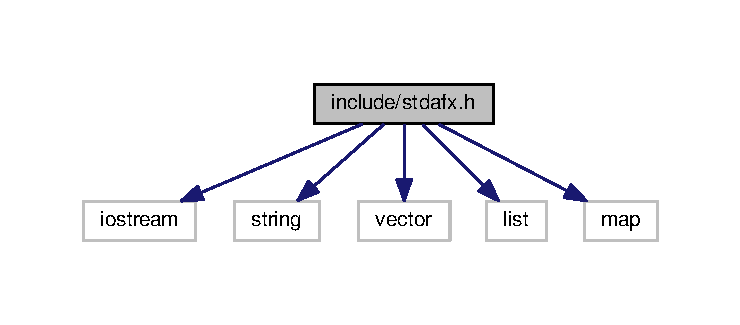
\includegraphics[width=350pt]{stdafx_8h__incl}
\end{center}
\end{figure}
This graph shows which files directly or indirectly include this file\-:
\nopagebreak
\begin{figure}[H]
\begin{center}
\leavevmode
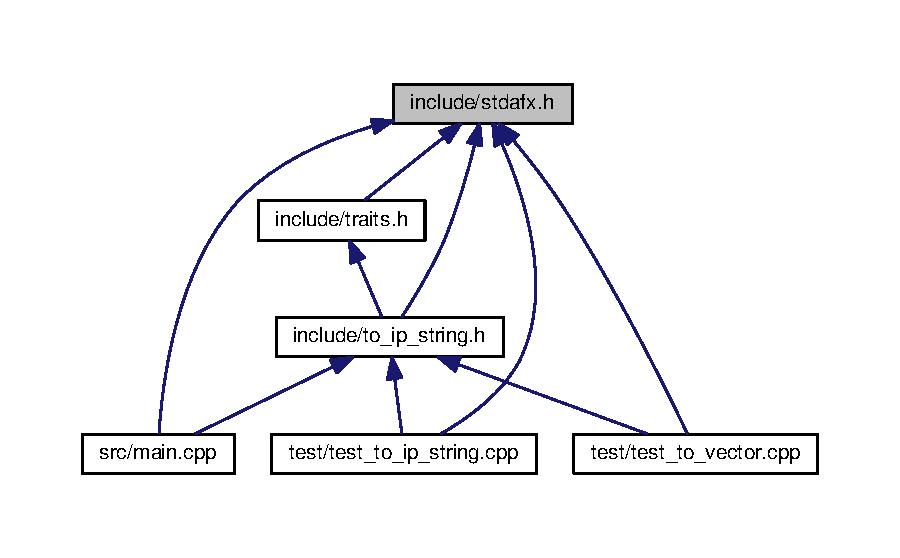
\includegraphics[width=322pt]{stdafx_8h__dep__incl}
\end{center}
\end{figure}

\hypertarget{to__ip__string_8h}{\section{include/to\-\_\-ip\-\_\-string.h File Reference}
\label{to__ip__string_8h}\index{include/to\-\_\-ip\-\_\-string.\-h@{include/to\-\_\-ip\-\_\-string.\-h}}
}
{\ttfamily \#include \char`\"{}stdafx.\-h\char`\"{}}\\*
{\ttfamily \#include \char`\"{}traits.\-h\char`\"{}}\\*
{\ttfamily \#include $<$utility$>$}\\*
{\ttfamily \#include $<$numeric$>$}\\*
Include dependency graph for to\-\_\-ip\-\_\-string.\-h\-:
\nopagebreak
\begin{figure}[H]
\begin{center}
\leavevmode
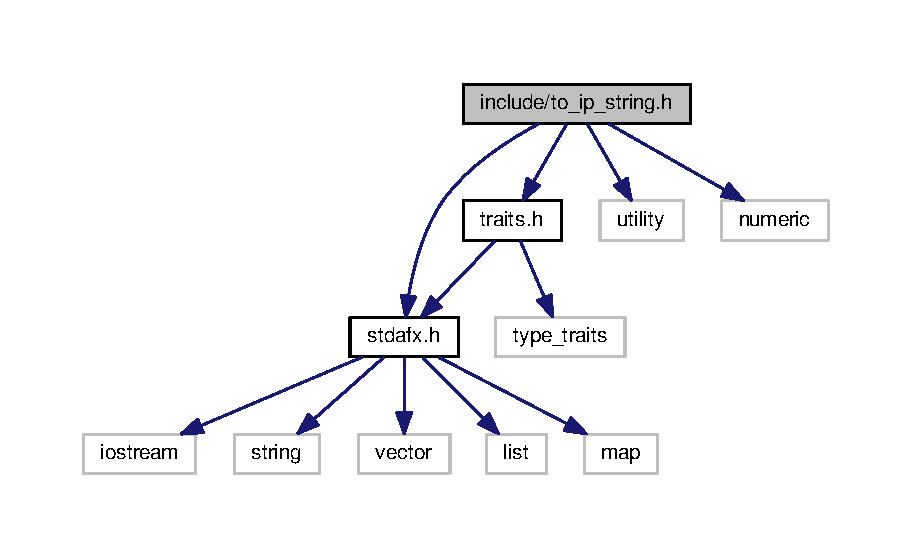
\includegraphics[width=350pt]{to__ip__string_8h__incl}
\end{center}
\end{figure}
This graph shows which files directly or indirectly include this file\-:
\nopagebreak
\begin{figure}[H]
\begin{center}
\leavevmode
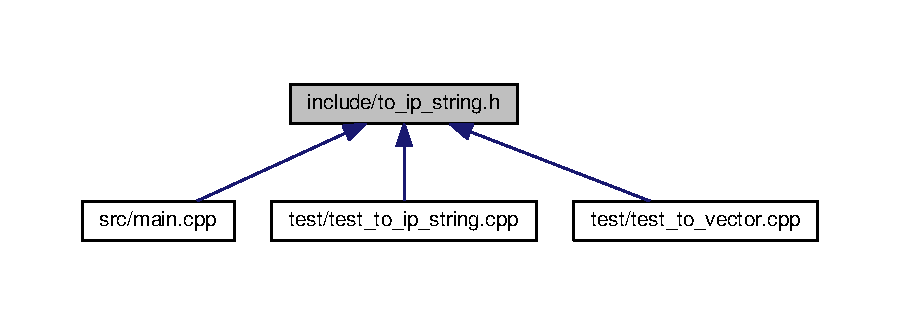
\includegraphics[width=350pt]{to__ip__string_8h__dep__incl}
\end{center}
\end{figure}
\subsection*{Functions}
\begin{DoxyCompactItemize}
\item 
{\footnotesize template$<$typename T , typename... T\-T$>$ }\\auto \hyperlink{to__ip__string_8h_a69f33ca1a20142e96a5cef2cb96c11ea}{to\-\_\-vector} (const std\-::tuple$<$ T, T\-T...$>$ \&in)
\item 
auto \hyperlink{to__ip__string_8h_a0846716611bb72a3092bcefcea9ac5f6}{to\-\_\-ip\-\_\-string} (const std\-::string in, bool is\-\_\-top=true)
\item 
{\footnotesize template$<$typename T $>$ }\\std\-::enable\-\_\-if\-\_\-t\\*
$<$ \hyperlink{traits_8h_afd5235ab6d17ce521e2312cc80a317f9}{is\-\_\-container\-\_\-v}$<$ T $>$\\*
 \&\&std\-::is\-\_\-same\-\_\-v$<$ typename \\*
T\-::value\-\_\-type, std\-::string $>$\\*
, std\-::string $>$ \hyperlink{to__ip__string_8h_aee52a715c042d3d454041021f267d035}{to\-\_\-ip\-\_\-string} (const T \&in, bool is\-\_\-top=true)
\item 
{\footnotesize template$<$typename T $>$ }\\std\-::enable\-\_\-if\-\_\-t\\*
$<$ std\-::is\-\_\-integral\-\_\-v$<$ T $>$\\*
, std\-::string $>$ \hyperlink{to__ip__string_8h_aa836169f7b430c6f32b67a950f04e476}{to\-\_\-ip\-\_\-string} (const T \&in, bool is\-\_\-top=true)
\item 
{\footnotesize template$<$typename T $>$ }\\std\-::enable\-\_\-if\-\_\-t\\*
$<$ \hyperlink{traits_8h_afd5235ab6d17ce521e2312cc80a317f9}{is\-\_\-container\-\_\-v}$<$ T $>$\\*
 \&\&!std\-::is\-\_\-same\-\_\-v$<$ typename \\*
T\-::value\-\_\-type, std\-::string $>$\\*
, std\-::string $>$ \hyperlink{to__ip__string_8h_a8b714168e352eeace458103a51a66dc8}{to\-\_\-ip\-\_\-string} (const T \&in, bool is\-\_\-top=true)
\item 
{\footnotesize template$<$typename... T$>$ }\\std\-::string \hyperlink{to__ip__string_8h_a4097b9037b4945c4a93c52fd46608486}{to\-\_\-ip\-\_\-string} (const std\-::tuple$<$ T...$>$ \&in, bool is\-\_\-top=true)
\item 
{\footnotesize template$<$typename T , typename Tuple , size\-\_\-t... Id$>$ }\\auto \hyperlink{to__ip__string_8h_a6f3ff16079c033a7dbc61506c1b87c90}{to\-\_\-vector\-\_\-impl} (const Tuple \&in, std\-::index\-\_\-sequence$<$ Id...$>$)
\item 
std\-::vector$<$ std\-::string $>$ \hyperlink{to__ip__string_8h_aabf6be604157bfb348556cea59d849fb}{to\-\_\-vector} (const std\-::tuple$<$$>$ \&in)
\end{DoxyCompactItemize}


\subsection{Function Documentation}
\hypertarget{to__ip__string_8h_a0846716611bb72a3092bcefcea9ac5f6}{\index{to\-\_\-ip\-\_\-string.\-h@{to\-\_\-ip\-\_\-string.\-h}!to\-\_\-ip\-\_\-string@{to\-\_\-ip\-\_\-string}}
\index{to\-\_\-ip\-\_\-string@{to\-\_\-ip\-\_\-string}!to_ip_string.h@{to\-\_\-ip\-\_\-string.\-h}}
\subsubsection[{to\-\_\-ip\-\_\-string}]{\setlength{\rightskip}{0pt plus 5cm}auto to\-\_\-ip\-\_\-string (
\begin{DoxyParamCaption}
\item[{const std\-::string}]{in, }
\item[{bool}]{is\-\_\-top = {\ttfamily true}}
\end{DoxyParamCaption}
)}}\label{to__ip__string_8h_a0846716611bb72a3092bcefcea9ac5f6}
\hypertarget{to__ip__string_8h_aee52a715c042d3d454041021f267d035}{\index{to\-\_\-ip\-\_\-string.\-h@{to\-\_\-ip\-\_\-string.\-h}!to\-\_\-ip\-\_\-string@{to\-\_\-ip\-\_\-string}}
\index{to\-\_\-ip\-\_\-string@{to\-\_\-ip\-\_\-string}!to_ip_string.h@{to\-\_\-ip\-\_\-string.\-h}}
\subsubsection[{to\-\_\-ip\-\_\-string}]{\setlength{\rightskip}{0pt plus 5cm}template$<$typename T $>$ std\-::enable\-\_\-if\-\_\-t$<$ {\bf is\-\_\-container\-\_\-v}$<$T$>$ \&\& std\-::is\-\_\-same\-\_\-v$<$typename T\-::value\-\_\-type, std\-::string$>$, std\-::string $>$ to\-\_\-ip\-\_\-string (
\begin{DoxyParamCaption}
\item[{const T \&}]{in, }
\item[{bool}]{is\-\_\-top = {\ttfamily true}}
\end{DoxyParamCaption}
)}}\label{to__ip__string_8h_aee52a715c042d3d454041021f267d035}
\hypertarget{to__ip__string_8h_aa836169f7b430c6f32b67a950f04e476}{\index{to\-\_\-ip\-\_\-string.\-h@{to\-\_\-ip\-\_\-string.\-h}!to\-\_\-ip\-\_\-string@{to\-\_\-ip\-\_\-string}}
\index{to\-\_\-ip\-\_\-string@{to\-\_\-ip\-\_\-string}!to_ip_string.h@{to\-\_\-ip\-\_\-string.\-h}}
\subsubsection[{to\-\_\-ip\-\_\-string}]{\setlength{\rightskip}{0pt plus 5cm}template$<$typename T $>$ std\-::enable\-\_\-if\-\_\-t$<$std\-::is\-\_\-integral\-\_\-v$<$T$>$, std\-::string $>$ to\-\_\-ip\-\_\-string (
\begin{DoxyParamCaption}
\item[{const T \&}]{in, }
\item[{bool}]{is\-\_\-top = {\ttfamily true}}
\end{DoxyParamCaption}
)}}\label{to__ip__string_8h_aa836169f7b430c6f32b67a950f04e476}
\hypertarget{to__ip__string_8h_a8b714168e352eeace458103a51a66dc8}{\index{to\-\_\-ip\-\_\-string.\-h@{to\-\_\-ip\-\_\-string.\-h}!to\-\_\-ip\-\_\-string@{to\-\_\-ip\-\_\-string}}
\index{to\-\_\-ip\-\_\-string@{to\-\_\-ip\-\_\-string}!to_ip_string.h@{to\-\_\-ip\-\_\-string.\-h}}
\subsubsection[{to\-\_\-ip\-\_\-string}]{\setlength{\rightskip}{0pt plus 5cm}template$<$typename T $>$ std\-::enable\-\_\-if\-\_\-t$<${\bf is\-\_\-container\-\_\-v}$<$T$>$ \&\& !std\-::is\-\_\-same\-\_\-v$<$typename T\-::value\-\_\-type, std\-::string$>$, std\-::string $>$ to\-\_\-ip\-\_\-string (
\begin{DoxyParamCaption}
\item[{const T \&}]{in, }
\item[{bool}]{is\-\_\-top = {\ttfamily true}}
\end{DoxyParamCaption}
)}}\label{to__ip__string_8h_a8b714168e352eeace458103a51a66dc8}
\hypertarget{to__ip__string_8h_a4097b9037b4945c4a93c52fd46608486}{\index{to\-\_\-ip\-\_\-string.\-h@{to\-\_\-ip\-\_\-string.\-h}!to\-\_\-ip\-\_\-string@{to\-\_\-ip\-\_\-string}}
\index{to\-\_\-ip\-\_\-string@{to\-\_\-ip\-\_\-string}!to_ip_string.h@{to\-\_\-ip\-\_\-string.\-h}}
\subsubsection[{to\-\_\-ip\-\_\-string}]{\setlength{\rightskip}{0pt plus 5cm}template$<$typename... T$>$ std\-::string to\-\_\-ip\-\_\-string (
\begin{DoxyParamCaption}
\item[{const std\-::tuple$<$ T...$>$ \&}]{in, }
\item[{bool}]{is\-\_\-top = {\ttfamily true}}
\end{DoxyParamCaption}
)}}\label{to__ip__string_8h_a4097b9037b4945c4a93c52fd46608486}
\hypertarget{to__ip__string_8h_a69f33ca1a20142e96a5cef2cb96c11ea}{\index{to\-\_\-ip\-\_\-string.\-h@{to\-\_\-ip\-\_\-string.\-h}!to\-\_\-vector@{to\-\_\-vector}}
\index{to\-\_\-vector@{to\-\_\-vector}!to_ip_string.h@{to\-\_\-ip\-\_\-string.\-h}}
\subsubsection[{to\-\_\-vector}]{\setlength{\rightskip}{0pt plus 5cm}template$<$typename T , typename... T\-T$>$ auto to\-\_\-vector (
\begin{DoxyParamCaption}
\item[{const std\-::tuple$<$ T, T\-T...$>$ \&}]{in}
\end{DoxyParamCaption}
)}}\label{to__ip__string_8h_a69f33ca1a20142e96a5cef2cb96c11ea}
\hypertarget{to__ip__string_8h_aabf6be604157bfb348556cea59d849fb}{\index{to\-\_\-ip\-\_\-string.\-h@{to\-\_\-ip\-\_\-string.\-h}!to\-\_\-vector@{to\-\_\-vector}}
\index{to\-\_\-vector@{to\-\_\-vector}!to_ip_string.h@{to\-\_\-ip\-\_\-string.\-h}}
\subsubsection[{to\-\_\-vector}]{\setlength{\rightskip}{0pt plus 5cm}std\-::vector$<$std\-::string$>$ to\-\_\-vector (
\begin{DoxyParamCaption}
\item[{const std\-::tuple$<$$>$ \&}]{in}
\end{DoxyParamCaption}
)}}\label{to__ip__string_8h_aabf6be604157bfb348556cea59d849fb}
\hypertarget{to__ip__string_8h_a6f3ff16079c033a7dbc61506c1b87c90}{\index{to\-\_\-ip\-\_\-string.\-h@{to\-\_\-ip\-\_\-string.\-h}!to\-\_\-vector\-\_\-impl@{to\-\_\-vector\-\_\-impl}}
\index{to\-\_\-vector\-\_\-impl@{to\-\_\-vector\-\_\-impl}!to_ip_string.h@{to\-\_\-ip\-\_\-string.\-h}}
\subsubsection[{to\-\_\-vector\-\_\-impl}]{\setlength{\rightskip}{0pt plus 5cm}template$<$typename T , typename Tuple , size\-\_\-t... Id$>$ auto to\-\_\-vector\-\_\-impl (
\begin{DoxyParamCaption}
\item[{const Tuple \&}]{in, }
\item[{std\-::index\-\_\-sequence$<$ Id...$>$}]{}
\end{DoxyParamCaption}
)}}\label{to__ip__string_8h_a6f3ff16079c033a7dbc61506c1b87c90}

\hypertarget{traits_8h}{\section{include/traits.h File Reference}
\label{traits_8h}\index{include/traits.\-h@{include/traits.\-h}}
}
{\ttfamily \#include \char`\"{}stdafx.\-h\char`\"{}}\\*
{\ttfamily \#include $<$type\-\_\-traits$>$}\\*
Include dependency graph for traits.\-h\-:
\nopagebreak
\begin{figure}[H]
\begin{center}
\leavevmode
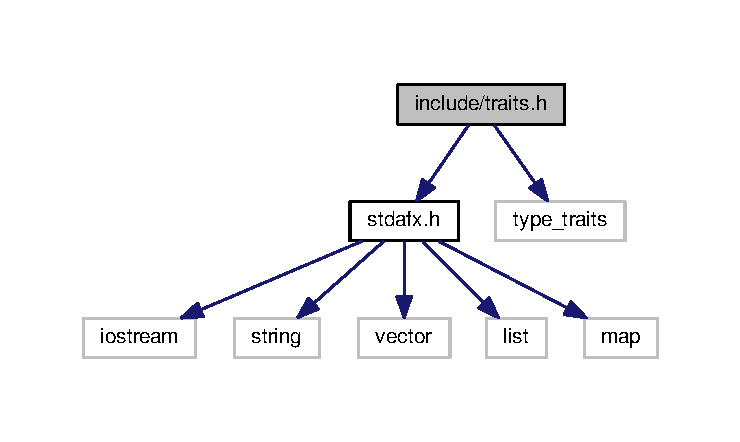
\includegraphics[width=350pt]{traits_8h__incl}
\end{center}
\end{figure}
This graph shows which files directly or indirectly include this file\-:
\nopagebreak
\begin{figure}[H]
\begin{center}
\leavevmode
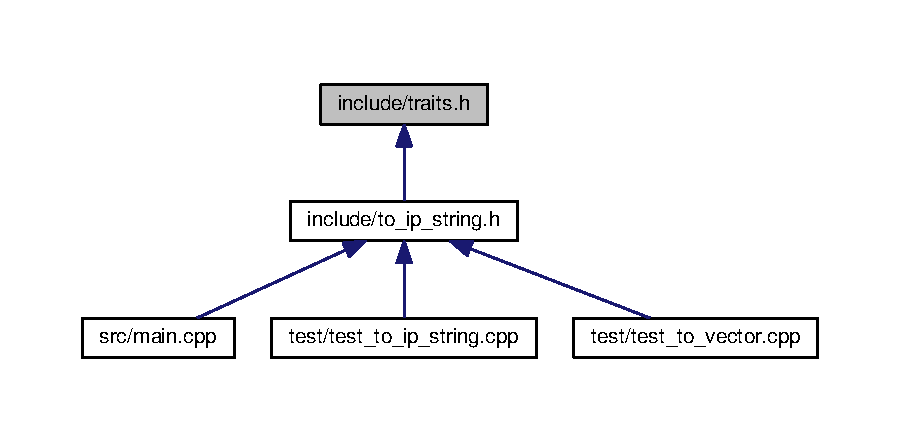
\includegraphics[width=350pt]{traits_8h__dep__incl}
\end{center}
\end{figure}
\subsection*{Classes}
\begin{DoxyCompactItemize}
\item 
struct \hyperlink{structis__container}{is\-\_\-container$<$ T, \-\_\- $>$}
\item 
struct \hyperlink{structis__container__helper}{is\-\_\-container\-\_\-helper$<$ Ts $>$}
\item 
struct \hyperlink{structis__container_3_01_t_00_01std_1_1conditional__t_3_01false_00_01is__container__helper_3_01te37159d0ff64b42c0f479ec01d5ef687}{conditional\-\_\-t$<$ false, is\-\_\-container\-\_\-helper$<$ typename T\-::value\-\_\-type, typename T\-::size\-\_\-type, typename T\-::allocator\-\_\-type, typename T\-::iterator, typename T\-::const\-\_\-iterator, decltype(std\-::declval$<$ T $>$().\-size()), decltype(std\-::declval$<$ T $>$().\-begin()), decltype(std\-::declval$<$ T $>$().\-end()), decltype(std\-::declval$<$ T $>$().\-cbegin()), decltype(std\-::declval$<$ T $>$().\-cend()) $>$, void $>$$>$}
\end{DoxyCompactItemize}
\subsection*{Variables}
\begin{DoxyCompactItemize}
\item 
{\footnotesize template$<$typename T $>$ }\\constexpr bool \hyperlink{traits_8h_afd5235ab6d17ce521e2312cc80a317f9}{is\-\_\-container\-\_\-v} = \hyperlink{structis__container}{is\-\_\-container}$<$T$>$\-::value
\end{DoxyCompactItemize}


\subsection{Variable Documentation}
\hypertarget{traits_8h_afd5235ab6d17ce521e2312cc80a317f9}{\index{traits.\-h@{traits.\-h}!is\-\_\-container\-\_\-v@{is\-\_\-container\-\_\-v}}
\index{is\-\_\-container\-\_\-v@{is\-\_\-container\-\_\-v}!traits.h@{traits.\-h}}
\subsubsection[{is\-\_\-container\-\_\-v}]{\setlength{\rightskip}{0pt plus 5cm}template$<$typename T $>$ constexpr bool is\-\_\-container\-\_\-v = {\bf is\-\_\-container}$<$T$>$\-::value}}\label{traits_8h_afd5235ab6d17ce521e2312cc80a317f9}

\hypertarget{_r_e_a_d_m_e_8md}{\section{R\-E\-A\-D\-M\-E.\-md File Reference}
\label{_r_e_a_d_m_e_8md}\index{R\-E\-A\-D\-M\-E.\-md@{R\-E\-A\-D\-M\-E.\-md}}
}

\hypertarget{main_8cpp}{\section{src/main.cpp File Reference}
\label{main_8cpp}\index{src/main.\-cpp@{src/main.\-cpp}}
}
{\ttfamily \#include \char`\"{}stdafx.\-h\char`\"{}}\\*
{\ttfamily \#include \char`\"{}foo.\-h\char`\"{}}\\*
Include dependency graph for main.\-cpp\-:
\nopagebreak
\begin{figure}[H]
\begin{center}
\leavevmode
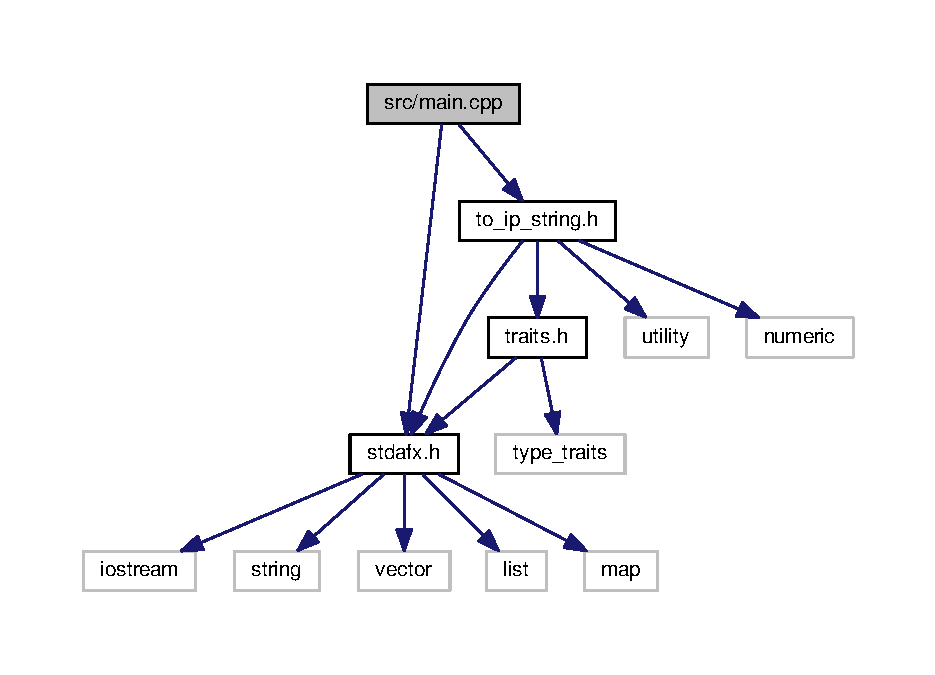
\includegraphics[width=350pt]{main_8cpp__incl}
\end{center}
\end{figure}
\subsection*{Functions}
\begin{DoxyCompactItemize}
\item 
int \hyperlink{main_8cpp_ae66f6b31b5ad750f1fe042a706a4e3d4}{main} ()
\end{DoxyCompactItemize}


\subsection{Function Documentation}
\hypertarget{main_8cpp_ae66f6b31b5ad750f1fe042a706a4e3d4}{\index{main.\-cpp@{main.\-cpp}!main@{main}}
\index{main@{main}!main.cpp@{main.\-cpp}}
\subsubsection[{main}]{\setlength{\rightskip}{0pt plus 5cm}int main (
\begin{DoxyParamCaption}
{}
\end{DoxyParamCaption}
)}}\label{main_8cpp_ae66f6b31b5ad750f1fe042a706a4e3d4}

\hypertarget{test__to__ip__string_8cpp}{\section{test/test\-\_\-to\-\_\-ip\-\_\-string.cpp File Reference}
\label{test__to__ip__string_8cpp}\index{test/test\-\_\-to\-\_\-ip\-\_\-string.\-cpp@{test/test\-\_\-to\-\_\-ip\-\_\-string.\-cpp}}
}
{\ttfamily \#include \char`\"{}../include/stdafx.\-h\char`\"{}}\\*
{\ttfamily \#include $<$boost/test/unit\-\_\-test.\-hpp$>$}\\*
{\ttfamily \#include \char`\"{}to\-\_\-ip\-\_\-string.\-h\char`\"{}}\\*
Include dependency graph for test\-\_\-to\-\_\-ip\-\_\-string.\-cpp\-:
\nopagebreak
\begin{figure}[H]
\begin{center}
\leavevmode
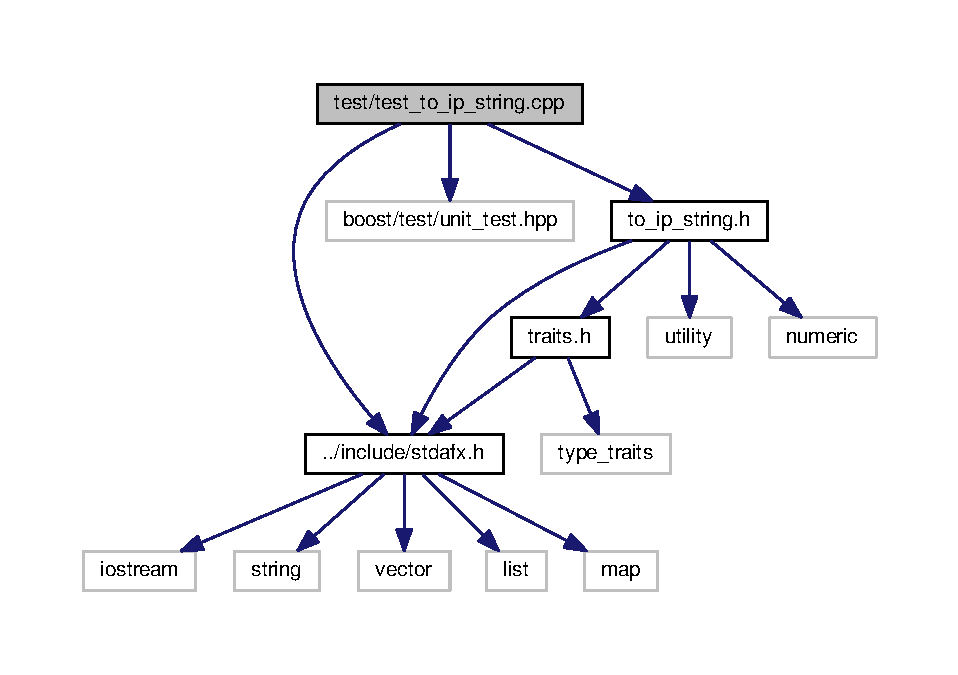
\includegraphics[width=350pt]{test__to__ip__string_8cpp__incl}
\end{center}
\end{figure}
\subsection*{Macros}
\begin{DoxyCompactItemize}
\item 
\#define \hyperlink{test__to__ip__string_8cpp_a6b2a3852db8bb19ab6909bac01859985}{B\-O\-O\-S\-T\-\_\-\-T\-E\-S\-T\-\_\-\-M\-O\-D\-U\-L\-E}~test\-\_\-foo
\item 
\#define \hyperlink{test__to__ip__string_8cpp_a0b87e0d3bf5853bcbb0b66a7c48fdc05}{L\-O\-G\-\_\-\-L\-E\-V\-E\-L}~all
\end{DoxyCompactItemize}
\subsection*{Functions}
\begin{DoxyCompactItemize}
\item 
\hyperlink{test__to__ip__string_8cpp_a1759e33433b036ab52c41af5bcdb0ad2}{B\-O\-O\-S\-T\-\_\-\-A\-U\-T\-O\-\_\-\-T\-E\-S\-T\-\_\-\-C\-A\-S\-E} (test\-\_\-to\-\_\-ip\-\_\-string\-\_\-\-\_\-base\-\_\-hw\-\_\-conversions)
\item 
\hyperlink{test__to__ip__string_8cpp_ae6124d4ce6026e820eef48b20e650824}{B\-O\-O\-S\-T\-\_\-\-A\-U\-T\-O\-\_\-\-T\-E\-S\-T\-\_\-\-C\-A\-S\-E} (test\-\_\-to\-\_\-ip\-\_\-string\-\_\-\-\_\-)
\end{DoxyCompactItemize}


\subsection{Macro Definition Documentation}
\hypertarget{test__to__ip__string_8cpp_a6b2a3852db8bb19ab6909bac01859985}{\index{test\-\_\-to\-\_\-ip\-\_\-string.\-cpp@{test\-\_\-to\-\_\-ip\-\_\-string.\-cpp}!B\-O\-O\-S\-T\-\_\-\-T\-E\-S\-T\-\_\-\-M\-O\-D\-U\-L\-E@{B\-O\-O\-S\-T\-\_\-\-T\-E\-S\-T\-\_\-\-M\-O\-D\-U\-L\-E}}
\index{B\-O\-O\-S\-T\-\_\-\-T\-E\-S\-T\-\_\-\-M\-O\-D\-U\-L\-E@{B\-O\-O\-S\-T\-\_\-\-T\-E\-S\-T\-\_\-\-M\-O\-D\-U\-L\-E}!test_to_ip_string.cpp@{test\-\_\-to\-\_\-ip\-\_\-string.\-cpp}}
\subsubsection[{B\-O\-O\-S\-T\-\_\-\-T\-E\-S\-T\-\_\-\-M\-O\-D\-U\-L\-E}]{\setlength{\rightskip}{0pt plus 5cm}\#define B\-O\-O\-S\-T\-\_\-\-T\-E\-S\-T\-\_\-\-M\-O\-D\-U\-L\-E~test\-\_\-foo}}\label{test__to__ip__string_8cpp_a6b2a3852db8bb19ab6909bac01859985}
\hypertarget{test__to__ip__string_8cpp_a0b87e0d3bf5853bcbb0b66a7c48fdc05}{\index{test\-\_\-to\-\_\-ip\-\_\-string.\-cpp@{test\-\_\-to\-\_\-ip\-\_\-string.\-cpp}!L\-O\-G\-\_\-\-L\-E\-V\-E\-L@{L\-O\-G\-\_\-\-L\-E\-V\-E\-L}}
\index{L\-O\-G\-\_\-\-L\-E\-V\-E\-L@{L\-O\-G\-\_\-\-L\-E\-V\-E\-L}!test_to_ip_string.cpp@{test\-\_\-to\-\_\-ip\-\_\-string.\-cpp}}
\subsubsection[{L\-O\-G\-\_\-\-L\-E\-V\-E\-L}]{\setlength{\rightskip}{0pt plus 5cm}\#define L\-O\-G\-\_\-\-L\-E\-V\-E\-L~all}}\label{test__to__ip__string_8cpp_a0b87e0d3bf5853bcbb0b66a7c48fdc05}


\subsection{Function Documentation}
\hypertarget{test__to__ip__string_8cpp_a1759e33433b036ab52c41af5bcdb0ad2}{\index{test\-\_\-to\-\_\-ip\-\_\-string.\-cpp@{test\-\_\-to\-\_\-ip\-\_\-string.\-cpp}!B\-O\-O\-S\-T\-\_\-\-A\-U\-T\-O\-\_\-\-T\-E\-S\-T\-\_\-\-C\-A\-S\-E@{B\-O\-O\-S\-T\-\_\-\-A\-U\-T\-O\-\_\-\-T\-E\-S\-T\-\_\-\-C\-A\-S\-E}}
\index{B\-O\-O\-S\-T\-\_\-\-A\-U\-T\-O\-\_\-\-T\-E\-S\-T\-\_\-\-C\-A\-S\-E@{B\-O\-O\-S\-T\-\_\-\-A\-U\-T\-O\-\_\-\-T\-E\-S\-T\-\_\-\-C\-A\-S\-E}!test_to_ip_string.cpp@{test\-\_\-to\-\_\-ip\-\_\-string.\-cpp}}
\subsubsection[{B\-O\-O\-S\-T\-\_\-\-A\-U\-T\-O\-\_\-\-T\-E\-S\-T\-\_\-\-C\-A\-S\-E}]{\setlength{\rightskip}{0pt plus 5cm}B\-O\-O\-S\-T\-\_\-\-A\-U\-T\-O\-\_\-\-T\-E\-S\-T\-\_\-\-C\-A\-S\-E (
\begin{DoxyParamCaption}
\item[{test\-\_\-to\-\_\-ip\-\_\-string\-\_\-\-\_\-base\-\_\-hw\-\_\-conversions}]{}
\end{DoxyParamCaption}
)}}\label{test__to__ip__string_8cpp_a1759e33433b036ab52c41af5bcdb0ad2}
\hypertarget{test__to__ip__string_8cpp_ae6124d4ce6026e820eef48b20e650824}{\index{test\-\_\-to\-\_\-ip\-\_\-string.\-cpp@{test\-\_\-to\-\_\-ip\-\_\-string.\-cpp}!B\-O\-O\-S\-T\-\_\-\-A\-U\-T\-O\-\_\-\-T\-E\-S\-T\-\_\-\-C\-A\-S\-E@{B\-O\-O\-S\-T\-\_\-\-A\-U\-T\-O\-\_\-\-T\-E\-S\-T\-\_\-\-C\-A\-S\-E}}
\index{B\-O\-O\-S\-T\-\_\-\-A\-U\-T\-O\-\_\-\-T\-E\-S\-T\-\_\-\-C\-A\-S\-E@{B\-O\-O\-S\-T\-\_\-\-A\-U\-T\-O\-\_\-\-T\-E\-S\-T\-\_\-\-C\-A\-S\-E}!test_to_ip_string.cpp@{test\-\_\-to\-\_\-ip\-\_\-string.\-cpp}}
\subsubsection[{B\-O\-O\-S\-T\-\_\-\-A\-U\-T\-O\-\_\-\-T\-E\-S\-T\-\_\-\-C\-A\-S\-E}]{\setlength{\rightskip}{0pt plus 5cm}B\-O\-O\-S\-T\-\_\-\-A\-U\-T\-O\-\_\-\-T\-E\-S\-T\-\_\-\-C\-A\-S\-E (
\begin{DoxyParamCaption}
\item[{test\-\_\-to\-\_\-ip\-\_\-string\-\_\-\-\_\-}]{}
\end{DoxyParamCaption}
)}}\label{test__to__ip__string_8cpp_ae6124d4ce6026e820eef48b20e650824}

\hypertarget{test__to__vector_8cpp}{\section{test/test\-\_\-to\-\_\-vector.cpp File Reference}
\label{test__to__vector_8cpp}\index{test/test\-\_\-to\-\_\-vector.\-cpp@{test/test\-\_\-to\-\_\-vector.\-cpp}}
}
{\ttfamily \#include \char`\"{}../include/stdafx.\-h\char`\"{}}\\*
{\ttfamily \#include $<$boost/test/unit\-\_\-test.\-hpp$>$}\\*
{\ttfamily \#include \char`\"{}to\-\_\-ip\-\_\-string.\-h\char`\"{}}\\*
Include dependency graph for test\-\_\-to\-\_\-vector.\-cpp\-:
\nopagebreak
\begin{figure}[H]
\begin{center}
\leavevmode
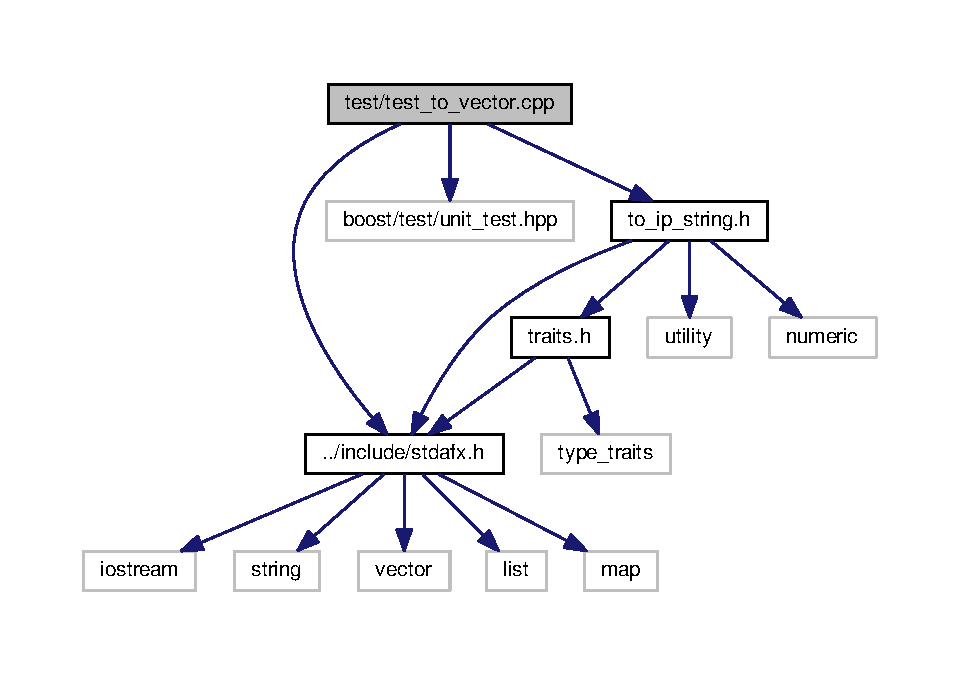
\includegraphics[width=350pt]{test__to__vector_8cpp__incl}
\end{center}
\end{figure}
\subsection*{Macros}
\begin{DoxyCompactItemize}
\item 
\#define \hyperlink{test__to__vector_8cpp_a6b2a3852db8bb19ab6909bac01859985}{B\-O\-O\-S\-T\-\_\-\-T\-E\-S\-T\-\_\-\-M\-O\-D\-U\-L\-E}~test\-\_\-foo
\item 
\#define \hyperlink{test__to__vector_8cpp_a0b87e0d3bf5853bcbb0b66a7c48fdc05}{L\-O\-G\-\_\-\-L\-E\-V\-E\-L}~all
\end{DoxyCompactItemize}
\subsection*{Functions}
\begin{DoxyCompactItemize}
\item 
\hyperlink{test__to__vector_8cpp_a8e766df196bd83ebcc86b3e2d8cd8d53}{B\-O\-O\-S\-T\-\_\-\-A\-U\-T\-O\-\_\-\-T\-E\-S\-T\-\_\-\-C\-A\-S\-E} (test\-\_\-to\-\_\-vector\-\_\-\-\_\-convert\-\_\-empty\-\_\-tuple)
\item 
\hyperlink{test__to__vector_8cpp_a229ead6ad657092c52b25e3677ceadb0}{B\-O\-O\-S\-T\-\_\-\-A\-U\-T\-O\-\_\-\-T\-E\-S\-T\-\_\-\-C\-A\-S\-E} (test\-\_\-to\-\_\-vector\-\_\-\-\_\-convert\-\_\-tuple\-\_\-of\-\_\-int)
\item 
\hyperlink{test__to__vector_8cpp_a8e5fb373ad68da33bd29c56349feb8aa}{B\-O\-O\-S\-T\-\_\-\-A\-U\-T\-O\-\_\-\-T\-E\-S\-T\-\_\-\-C\-A\-S\-E} (test\-\_\-to\-\_\-vector\-\_\-\-\_\-convert\-\_\-tuple\-\_\-of\-\_\-diff\-\_\-types)
\end{DoxyCompactItemize}


\subsection{Macro Definition Documentation}
\hypertarget{test__to__vector_8cpp_a6b2a3852db8bb19ab6909bac01859985}{\index{test\-\_\-to\-\_\-vector.\-cpp@{test\-\_\-to\-\_\-vector.\-cpp}!B\-O\-O\-S\-T\-\_\-\-T\-E\-S\-T\-\_\-\-M\-O\-D\-U\-L\-E@{B\-O\-O\-S\-T\-\_\-\-T\-E\-S\-T\-\_\-\-M\-O\-D\-U\-L\-E}}
\index{B\-O\-O\-S\-T\-\_\-\-T\-E\-S\-T\-\_\-\-M\-O\-D\-U\-L\-E@{B\-O\-O\-S\-T\-\_\-\-T\-E\-S\-T\-\_\-\-M\-O\-D\-U\-L\-E}!test_to_vector.cpp@{test\-\_\-to\-\_\-vector.\-cpp}}
\subsubsection[{B\-O\-O\-S\-T\-\_\-\-T\-E\-S\-T\-\_\-\-M\-O\-D\-U\-L\-E}]{\setlength{\rightskip}{0pt plus 5cm}\#define B\-O\-O\-S\-T\-\_\-\-T\-E\-S\-T\-\_\-\-M\-O\-D\-U\-L\-E~test\-\_\-foo}}\label{test__to__vector_8cpp_a6b2a3852db8bb19ab6909bac01859985}
\hypertarget{test__to__vector_8cpp_a0b87e0d3bf5853bcbb0b66a7c48fdc05}{\index{test\-\_\-to\-\_\-vector.\-cpp@{test\-\_\-to\-\_\-vector.\-cpp}!L\-O\-G\-\_\-\-L\-E\-V\-E\-L@{L\-O\-G\-\_\-\-L\-E\-V\-E\-L}}
\index{L\-O\-G\-\_\-\-L\-E\-V\-E\-L@{L\-O\-G\-\_\-\-L\-E\-V\-E\-L}!test_to_vector.cpp@{test\-\_\-to\-\_\-vector.\-cpp}}
\subsubsection[{L\-O\-G\-\_\-\-L\-E\-V\-E\-L}]{\setlength{\rightskip}{0pt plus 5cm}\#define L\-O\-G\-\_\-\-L\-E\-V\-E\-L~all}}\label{test__to__vector_8cpp_a0b87e0d3bf5853bcbb0b66a7c48fdc05}


\subsection{Function Documentation}
\hypertarget{test__to__vector_8cpp_a8e766df196bd83ebcc86b3e2d8cd8d53}{\index{test\-\_\-to\-\_\-vector.\-cpp@{test\-\_\-to\-\_\-vector.\-cpp}!B\-O\-O\-S\-T\-\_\-\-A\-U\-T\-O\-\_\-\-T\-E\-S\-T\-\_\-\-C\-A\-S\-E@{B\-O\-O\-S\-T\-\_\-\-A\-U\-T\-O\-\_\-\-T\-E\-S\-T\-\_\-\-C\-A\-S\-E}}
\index{B\-O\-O\-S\-T\-\_\-\-A\-U\-T\-O\-\_\-\-T\-E\-S\-T\-\_\-\-C\-A\-S\-E@{B\-O\-O\-S\-T\-\_\-\-A\-U\-T\-O\-\_\-\-T\-E\-S\-T\-\_\-\-C\-A\-S\-E}!test_to_vector.cpp@{test\-\_\-to\-\_\-vector.\-cpp}}
\subsubsection[{B\-O\-O\-S\-T\-\_\-\-A\-U\-T\-O\-\_\-\-T\-E\-S\-T\-\_\-\-C\-A\-S\-E}]{\setlength{\rightskip}{0pt plus 5cm}B\-O\-O\-S\-T\-\_\-\-A\-U\-T\-O\-\_\-\-T\-E\-S\-T\-\_\-\-C\-A\-S\-E (
\begin{DoxyParamCaption}
\item[{test\-\_\-to\-\_\-vector\-\_\-\-\_\-convert\-\_\-empty\-\_\-tuple}]{}
\end{DoxyParamCaption}
)}}\label{test__to__vector_8cpp_a8e766df196bd83ebcc86b3e2d8cd8d53}
\hypertarget{test__to__vector_8cpp_a229ead6ad657092c52b25e3677ceadb0}{\index{test\-\_\-to\-\_\-vector.\-cpp@{test\-\_\-to\-\_\-vector.\-cpp}!B\-O\-O\-S\-T\-\_\-\-A\-U\-T\-O\-\_\-\-T\-E\-S\-T\-\_\-\-C\-A\-S\-E@{B\-O\-O\-S\-T\-\_\-\-A\-U\-T\-O\-\_\-\-T\-E\-S\-T\-\_\-\-C\-A\-S\-E}}
\index{B\-O\-O\-S\-T\-\_\-\-A\-U\-T\-O\-\_\-\-T\-E\-S\-T\-\_\-\-C\-A\-S\-E@{B\-O\-O\-S\-T\-\_\-\-A\-U\-T\-O\-\_\-\-T\-E\-S\-T\-\_\-\-C\-A\-S\-E}!test_to_vector.cpp@{test\-\_\-to\-\_\-vector.\-cpp}}
\subsubsection[{B\-O\-O\-S\-T\-\_\-\-A\-U\-T\-O\-\_\-\-T\-E\-S\-T\-\_\-\-C\-A\-S\-E}]{\setlength{\rightskip}{0pt plus 5cm}B\-O\-O\-S\-T\-\_\-\-A\-U\-T\-O\-\_\-\-T\-E\-S\-T\-\_\-\-C\-A\-S\-E (
\begin{DoxyParamCaption}
\item[{test\-\_\-to\-\_\-vector\-\_\-\-\_\-convert\-\_\-tuple\-\_\-of\-\_\-int}]{}
\end{DoxyParamCaption}
)}}\label{test__to__vector_8cpp_a229ead6ad657092c52b25e3677ceadb0}
\hypertarget{test__to__vector_8cpp_a8e5fb373ad68da33bd29c56349feb8aa}{\index{test\-\_\-to\-\_\-vector.\-cpp@{test\-\_\-to\-\_\-vector.\-cpp}!B\-O\-O\-S\-T\-\_\-\-A\-U\-T\-O\-\_\-\-T\-E\-S\-T\-\_\-\-C\-A\-S\-E@{B\-O\-O\-S\-T\-\_\-\-A\-U\-T\-O\-\_\-\-T\-E\-S\-T\-\_\-\-C\-A\-S\-E}}
\index{B\-O\-O\-S\-T\-\_\-\-A\-U\-T\-O\-\_\-\-T\-E\-S\-T\-\_\-\-C\-A\-S\-E@{B\-O\-O\-S\-T\-\_\-\-A\-U\-T\-O\-\_\-\-T\-E\-S\-T\-\_\-\-C\-A\-S\-E}!test_to_vector.cpp@{test\-\_\-to\-\_\-vector.\-cpp}}
\subsubsection[{B\-O\-O\-S\-T\-\_\-\-A\-U\-T\-O\-\_\-\-T\-E\-S\-T\-\_\-\-C\-A\-S\-E}]{\setlength{\rightskip}{0pt plus 5cm}B\-O\-O\-S\-T\-\_\-\-A\-U\-T\-O\-\_\-\-T\-E\-S\-T\-\_\-\-C\-A\-S\-E (
\begin{DoxyParamCaption}
\item[{test\-\_\-to\-\_\-vector\-\_\-\-\_\-convert\-\_\-tuple\-\_\-of\-\_\-diff\-\_\-types}]{}
\end{DoxyParamCaption}
)}}\label{test__to__vector_8cpp_a8e5fb373ad68da33bd29c56349feb8aa}

%--- End generated contents ---

% Index
\newpage
\phantomsection
\addcontentsline{toc}{chapter}{Index}
\printindex

\end{document}
